\chapter{System Modeling}
\section{Activity Diagram}

\begin{figure}[H]
    \centering
    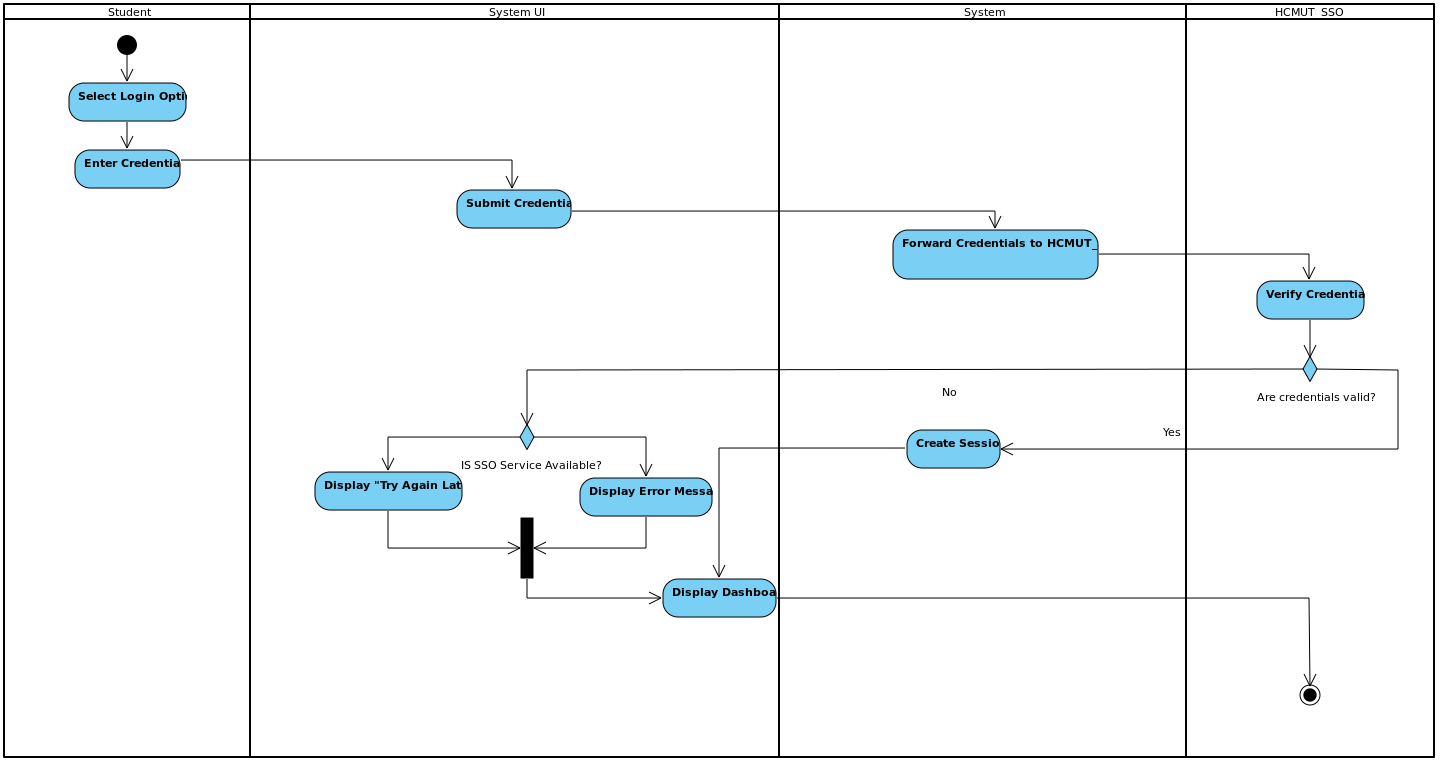
\includegraphics[width = 5in]{activity_diagram/login.png}
    \caption{UseCase - Login}
\end{figure}

This diagram illustrates the login process for a student accessing the HCMUT Student Smart Printing Service (HCMUT\_SSPS) through the HCMUT Single Sign-On (SSO) authentication service.

The process begins when a Student selects the login option and enters their credentials. These credentials are then submitted through the System UI, which forwards them to the System and subsequently to the HCMUT SSO service.

In the HCMUT SSO lane, the credentials are verified. If the credentials are invalid, the process will terminate with an error message displayed back to the user. If the credentials are valid, the System creates a session for the user, enabling successful login. If there are issues connecting to the SSO service, an error or "try again later" message is displayed to the student. If successful, the Dashboard is displayed to the user, concluding the login process.

This diagram covers key decision points, such as credential validity checks and service availability, to handle different scenarios in the login workflow.

\begin{figure}[H]
    \centering
    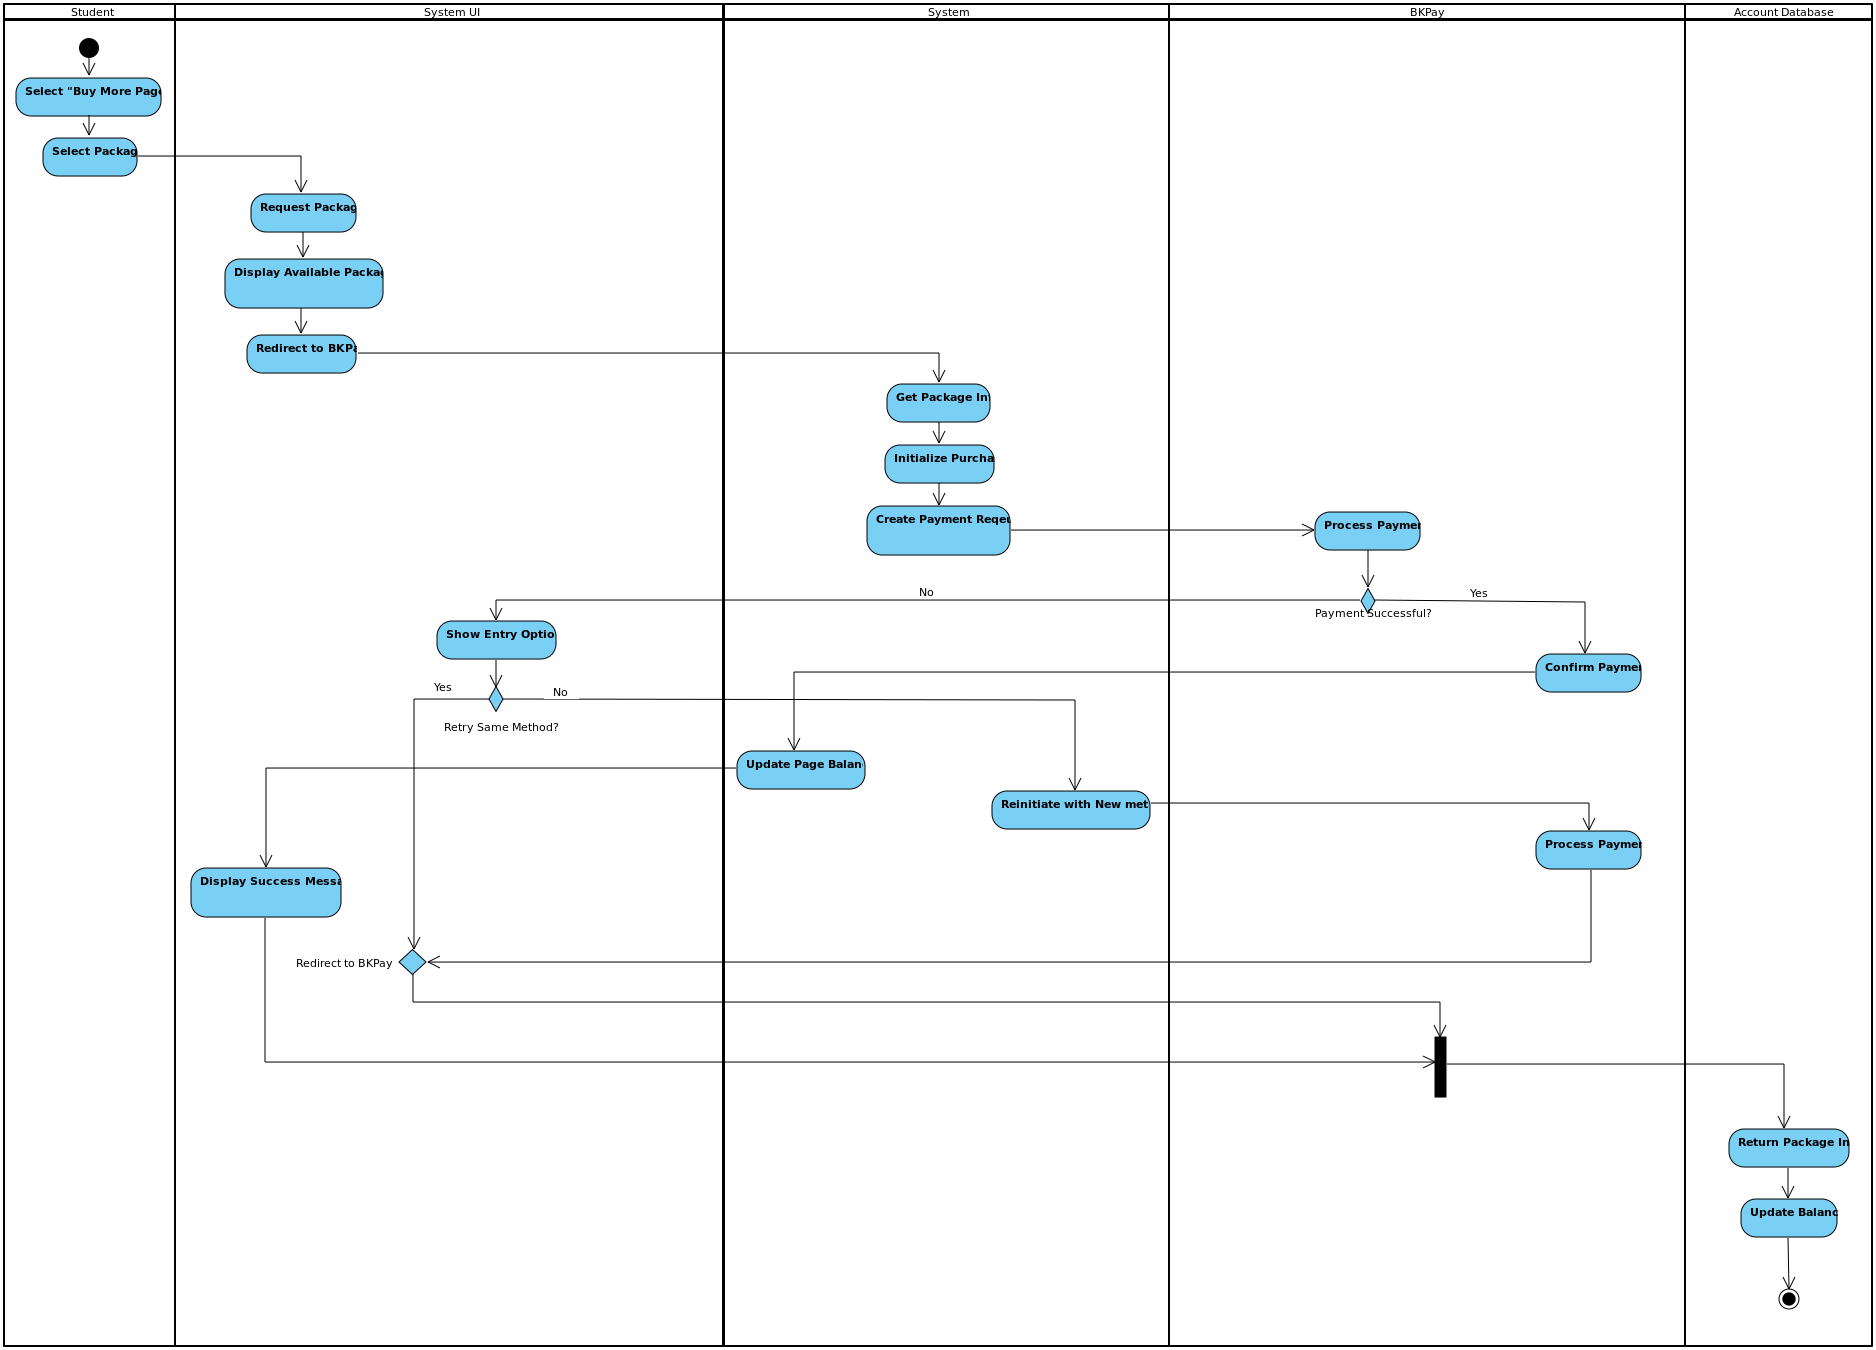
\includegraphics[width = 5in]{activity_diagram/buy_more_pages.png}
    \caption{UseCase - Buy More Pages}
\end{figure}
This diagram outlines the workflow of purchasing additional printing pages in the HCMUT Student Smart Printing Service. The process starts when a student initiates the "Buy More Pages" action, selects a desired package, and is redirected to BKPay for payment processing. After the System retrieves package details and prepares a payment request, the BKPay service processes the payment. If the payment is successful, the System updates the student’s page balance and displays a success message. If the payment fails, the student is given options to retry or select a different payment method. The diagram captures essential decision points, error handling, and system interactions to ensure the smooth completion of the purchase process, helping students conveniently manage their printing needs.

\begin{figure}[H]
    \centering
    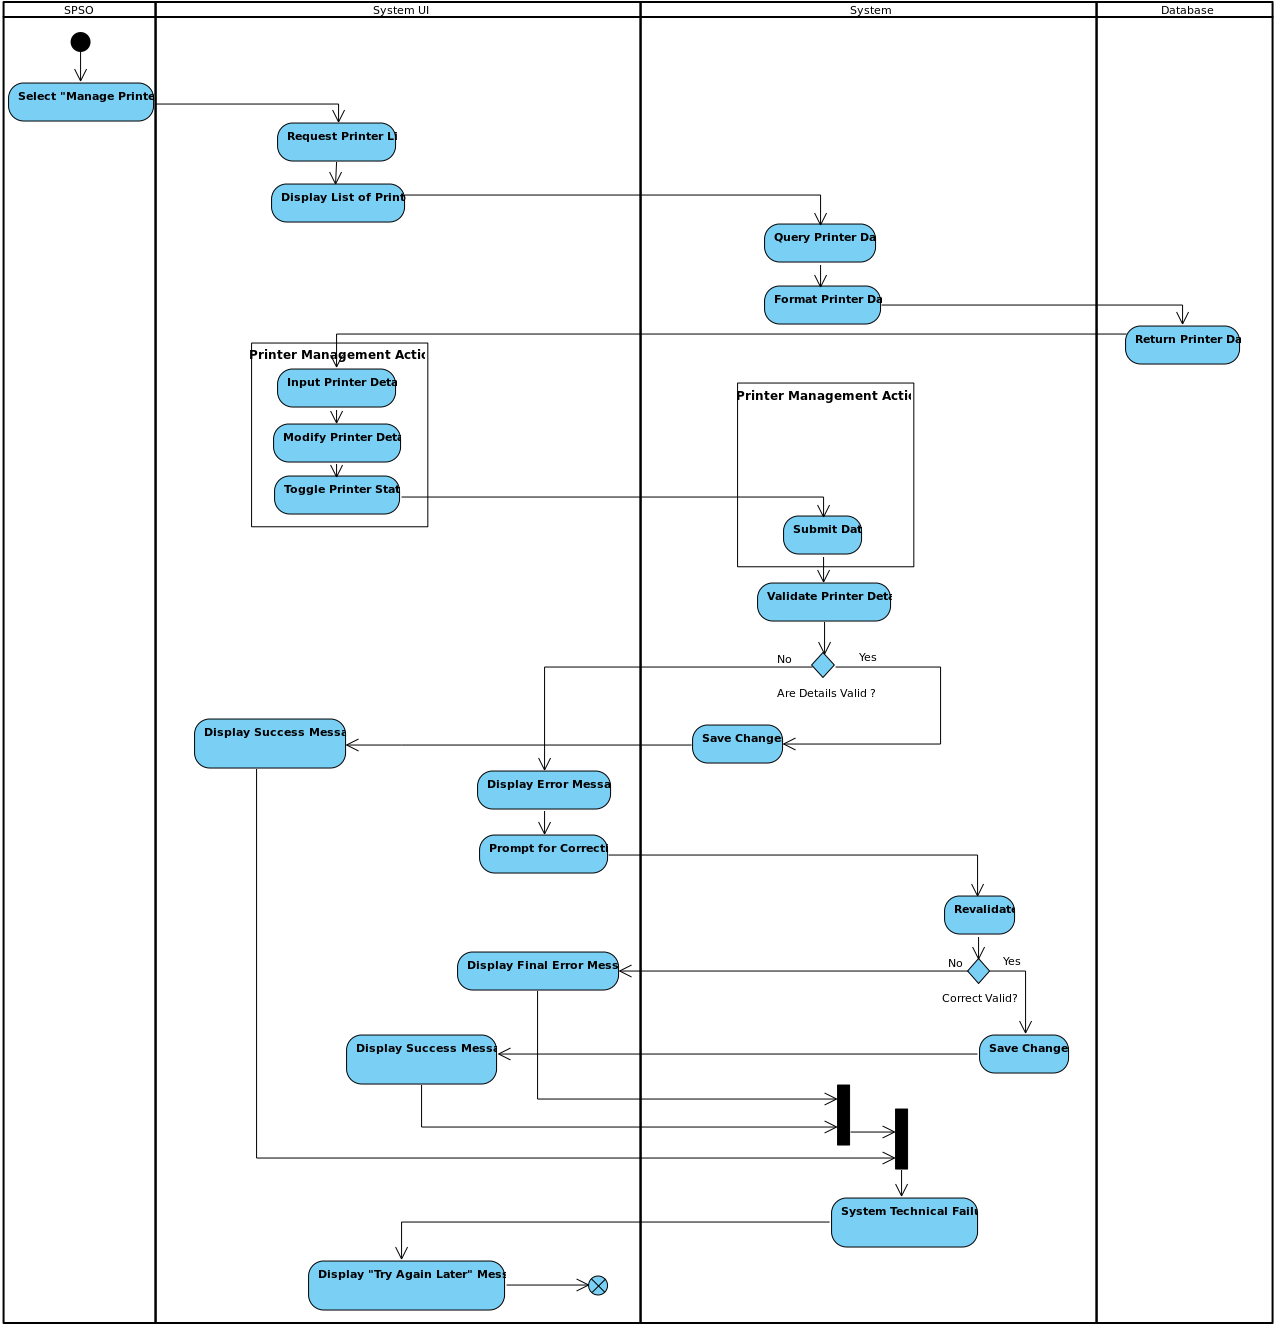
\includegraphics[width = 5in]{activity_diagram/manage_printers.png}
    \caption{UseCase - Manage Printers}
\end{figure}
This diagram illustrates the process of managing printers within the HCMUT Student Smart Printing Service by the Student Printing Service Officer (SPSO).

The process starts when the SPSO selects the "Manage Printers" option. The System UI requests and displays a list of available printers by querying the System and retrieving data from the Database. The SPSO can then perform various printer management actions, such as entering new printer details, modifying existing printer information, or toggling a printer's status (e.g., enabling or disabling a printer).

When the SPSO submits printer information, the System validates the input details. If there are errors, an error message is displayed and the SPSO is prompted to correct the details. If the validation fails repeatedly, a final error message is displayed. Once validated, changes are saved and a success message confirms the update. In case of a technical failure during the process, the system displays a "Try Again Later" message to the SPSO, allowing them to retry at a later time.

This diagram captures the detailed workflow for printer management, including decision points for validation, error handling, and the steps to successfully update printer settings in the system.


\begin{figure}[H]
    \centering
    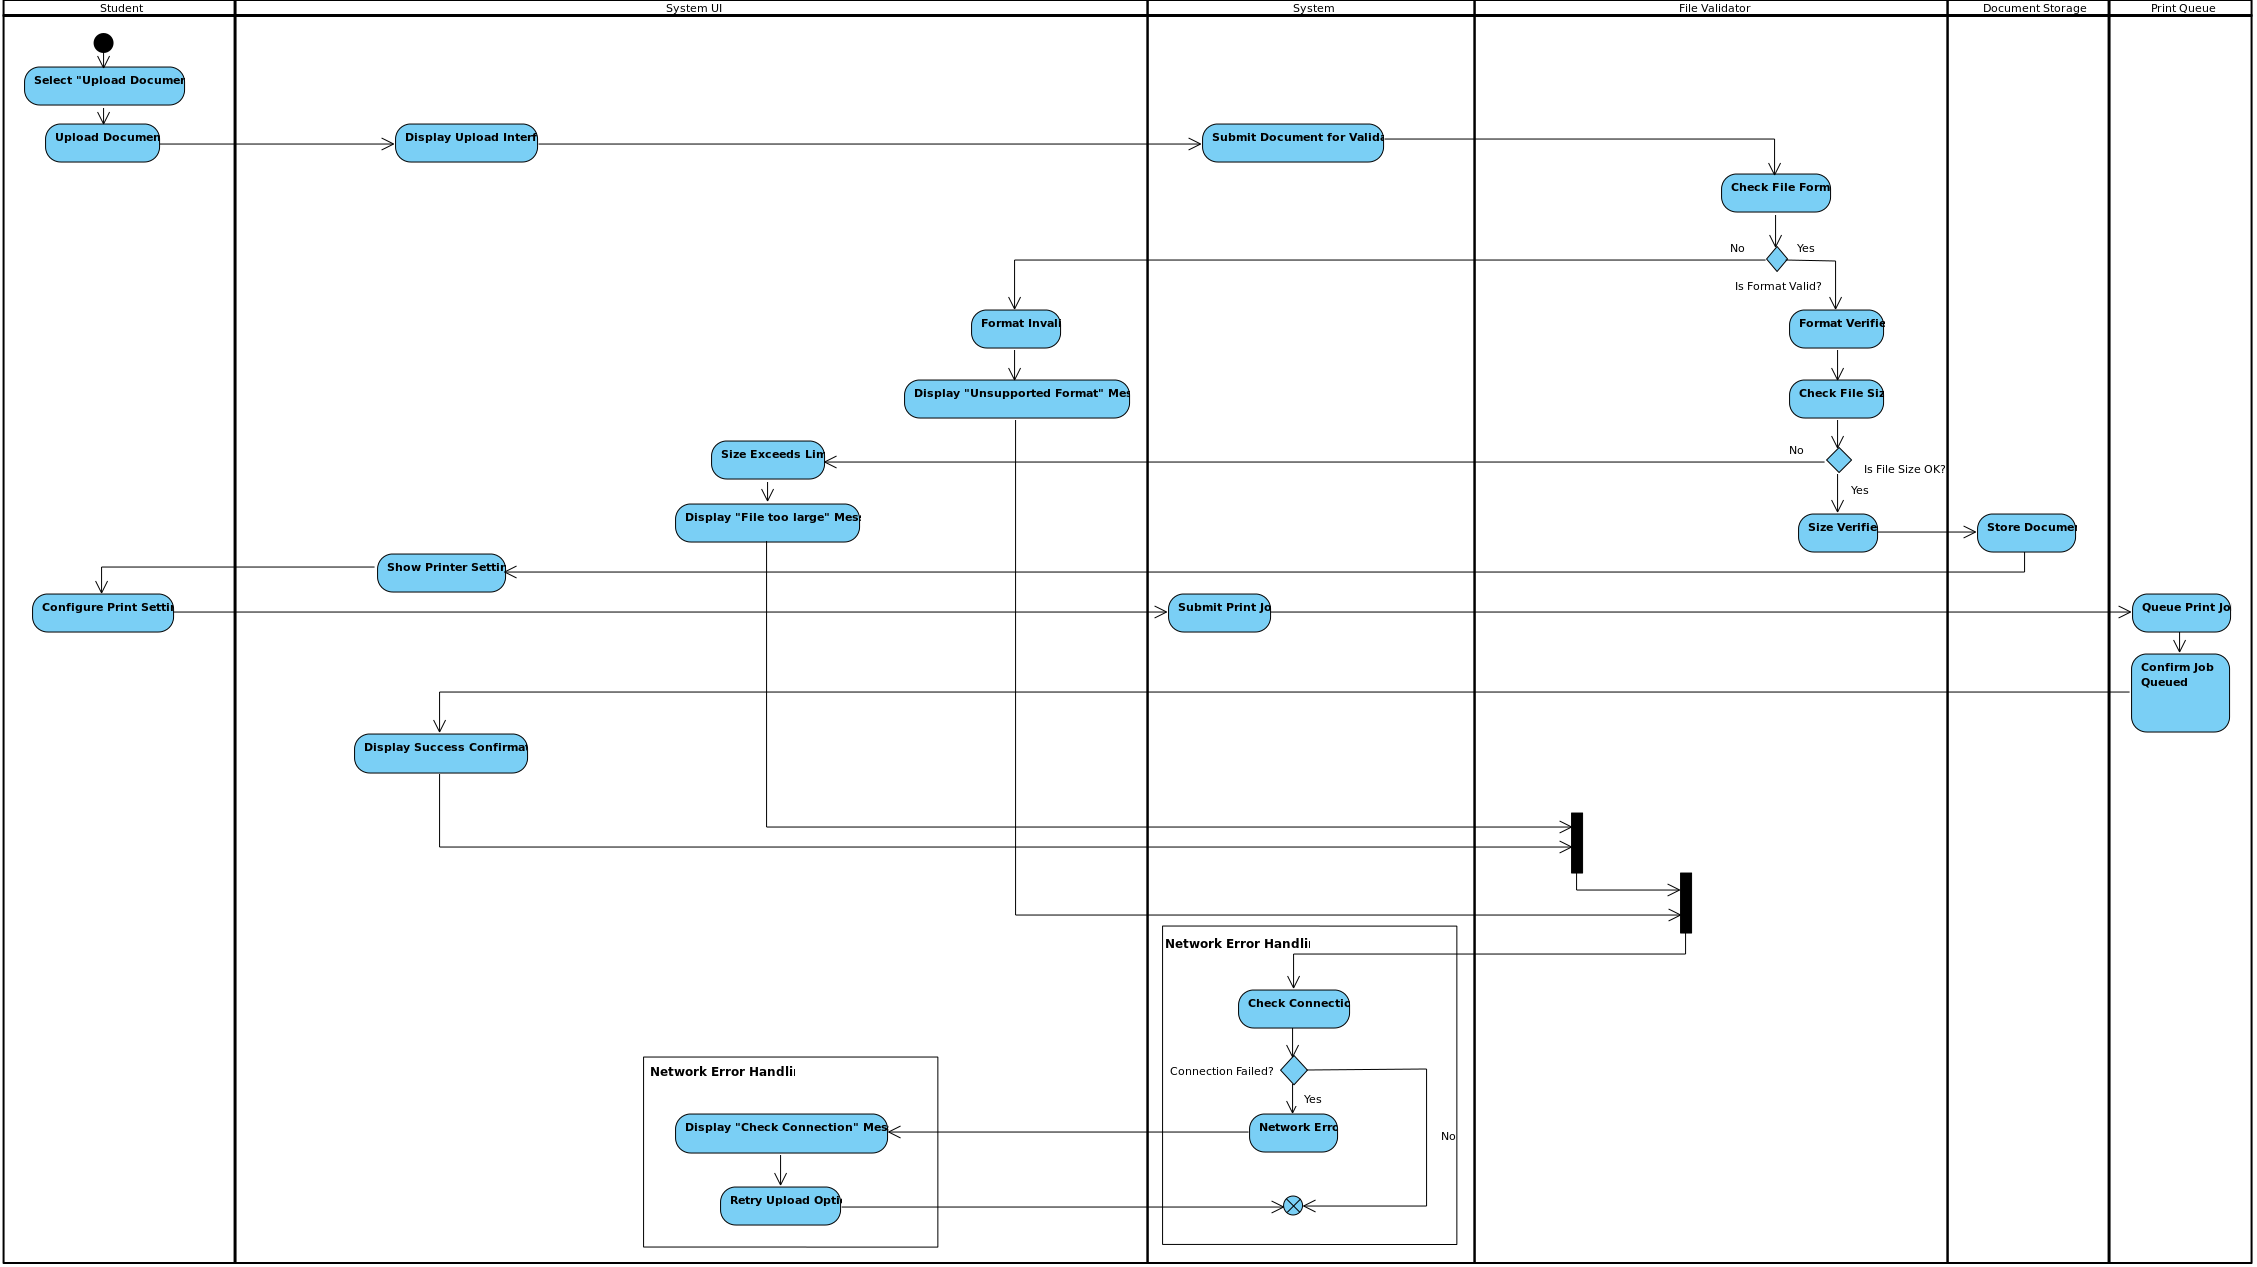
\includegraphics[width = 5in]{activity_diagram/upload_docs.png}
    \caption{UseCase - Upload Docs}
\end{figure}
This Activity Diagram illustrates the document upload and printing process in the HCMUT Student Smart Printing Service. 

The process begins with a Student selecting the "Upload Document" option and uploading their document through the System UI. The System forwards the document to the File Validator to check the file format and size. If the format is unsupported, an "Unsupported Format" message is displayed. If the file size exceeds the limit, a "File Too Large" message is shown, and the student must modify the file before retrying.

Once the file passes validation for both format and size, it is stored in Document Storage. The System UI then allows the student to configure print settings (e.g., paper size, print quality, and copies). After the student confirms the print settings, the System submits the print job to the Print Queue.
The print job is then queued, and a confirmation message is displayed, indicating that the job has been successfully queued for printing. In case of a network error during upload, the Network Error Handling process prompts the student to check their connection and retry the upload.

This diagram captures essential decision points, validation steps, and error-handling mechanisms to ensure a smooth and efficient document upload and printing process for students.

\begin{figure}[H]
    \centering
    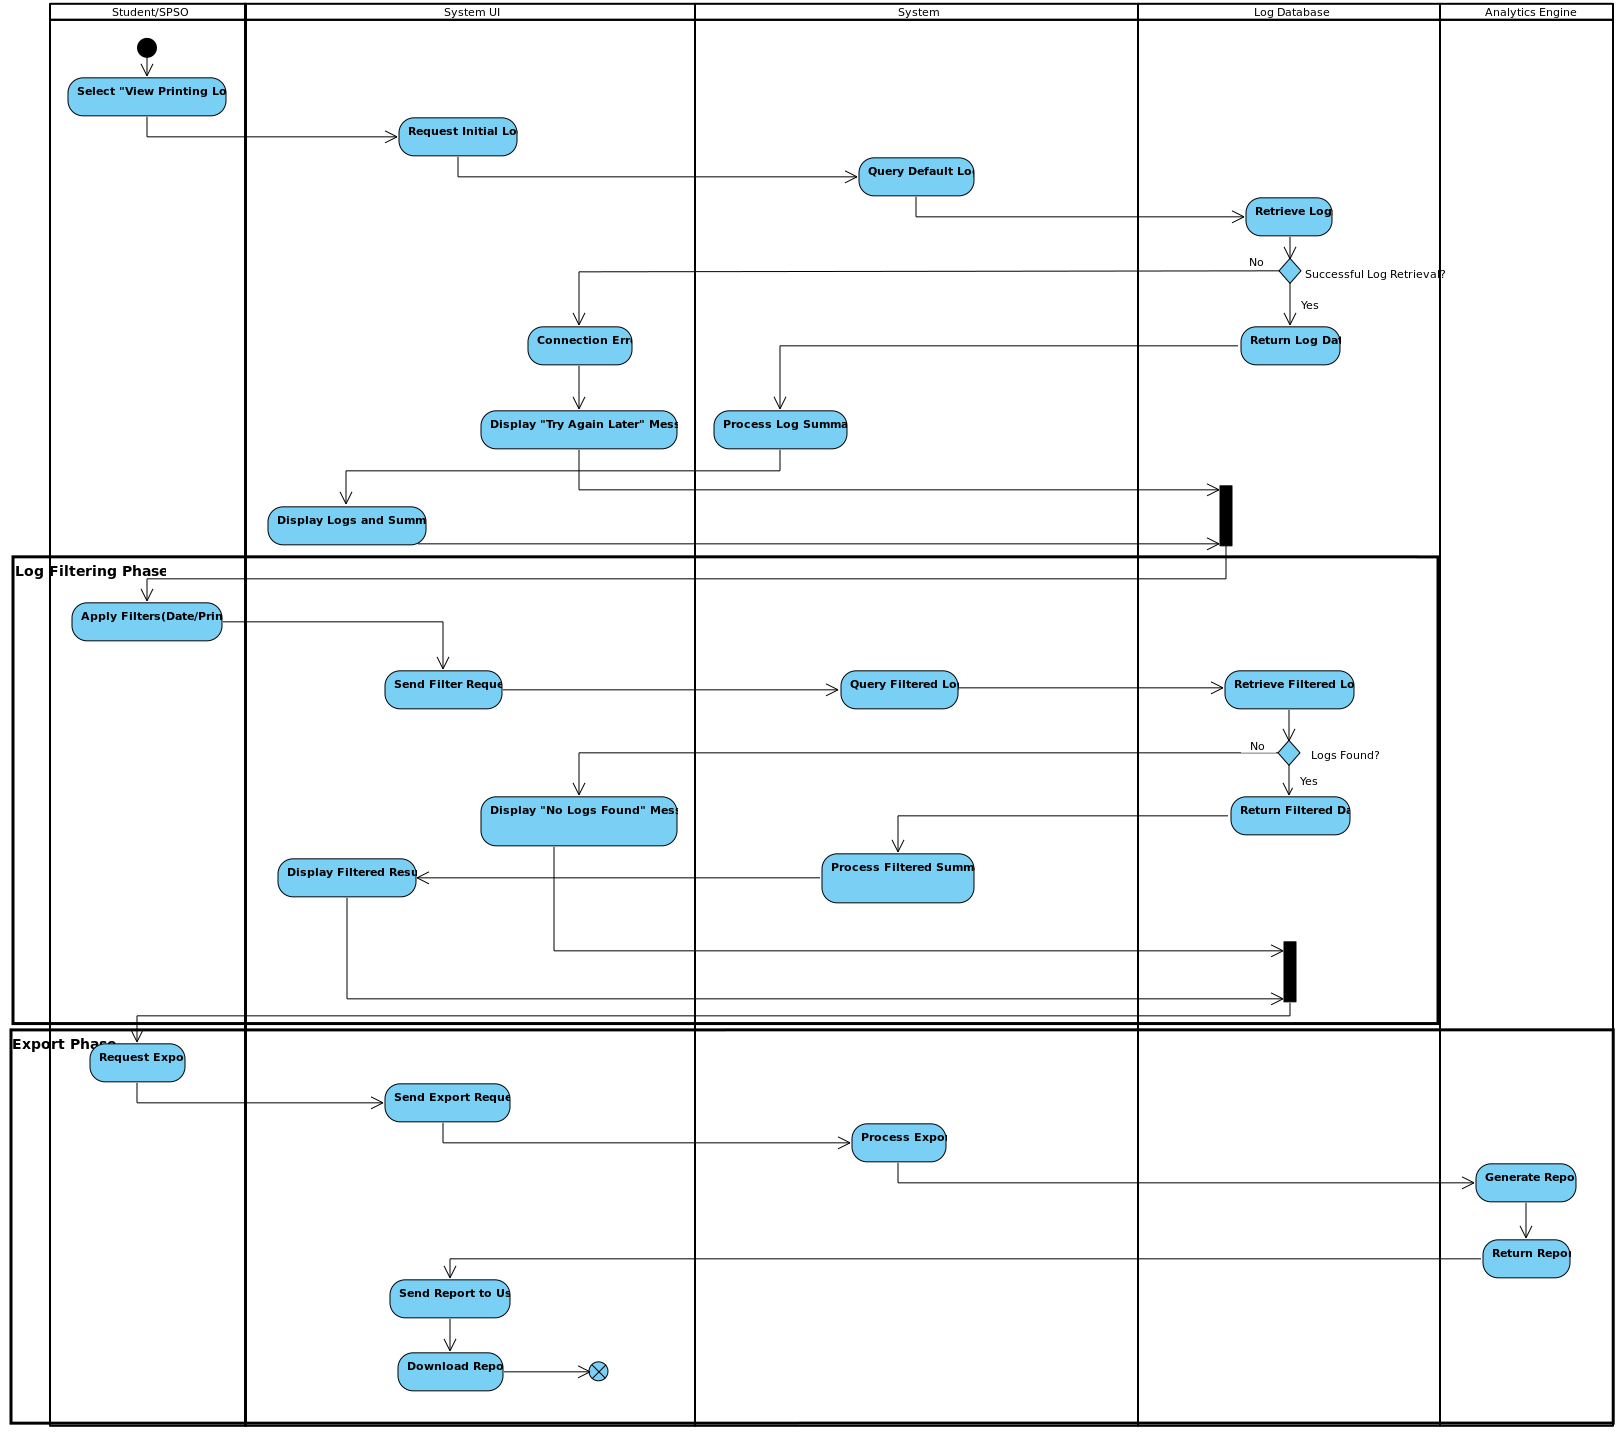
\includegraphics[width = 5in]{activity_diagram/view_printing_logs.png}
    \caption{UseCase - View Printing Logs}
\end{figure}
This Activity Diagram illustrates the process of viewing, filtering, and exporting printing logs within the HCMUT Student Smart Printing Service. Both Students and Student Printing Service Officers (SPSO) can access this feature.
\begin{enumerate}
    \item The process begins when a user selects "View Printing Logs." The System UI requests the initial logs, and the System queries the Log Database for default log data. If retrieval is successful, the logs and a summary are displayed. If there is a connection error, an error message prompts the user to try again later.
    \item In the Log Filtering Phase, the user applies specific filters (such as date, printer ID, or student ID). The System processes the filter request, queries the Log Database for the filtered data, and checks if any logs match the filters. If no logs are found, a "No Logs Found" message is displayed; otherwise, the filtered results and summary are shown.
    \item In the Export Phase, the user can request an export of the filtered or full log data. The System processes this request and generates a report through the Analytics Engine. The generated report is then made available for download, allowing the user to retrieve a detailed log record.
\end{enumerate}
This diagram captures the steps, decision points, and error-handling mechanisms involved in accessing and managing printing logs, giving users flexible options to view, filter, and export data as needed.


\section{Sequence Diagram}

\subsection{Usecase Login}

\vspace{1cm}

\begin{figure}[H]
    \vspace{-0.5cm}
    \centering
    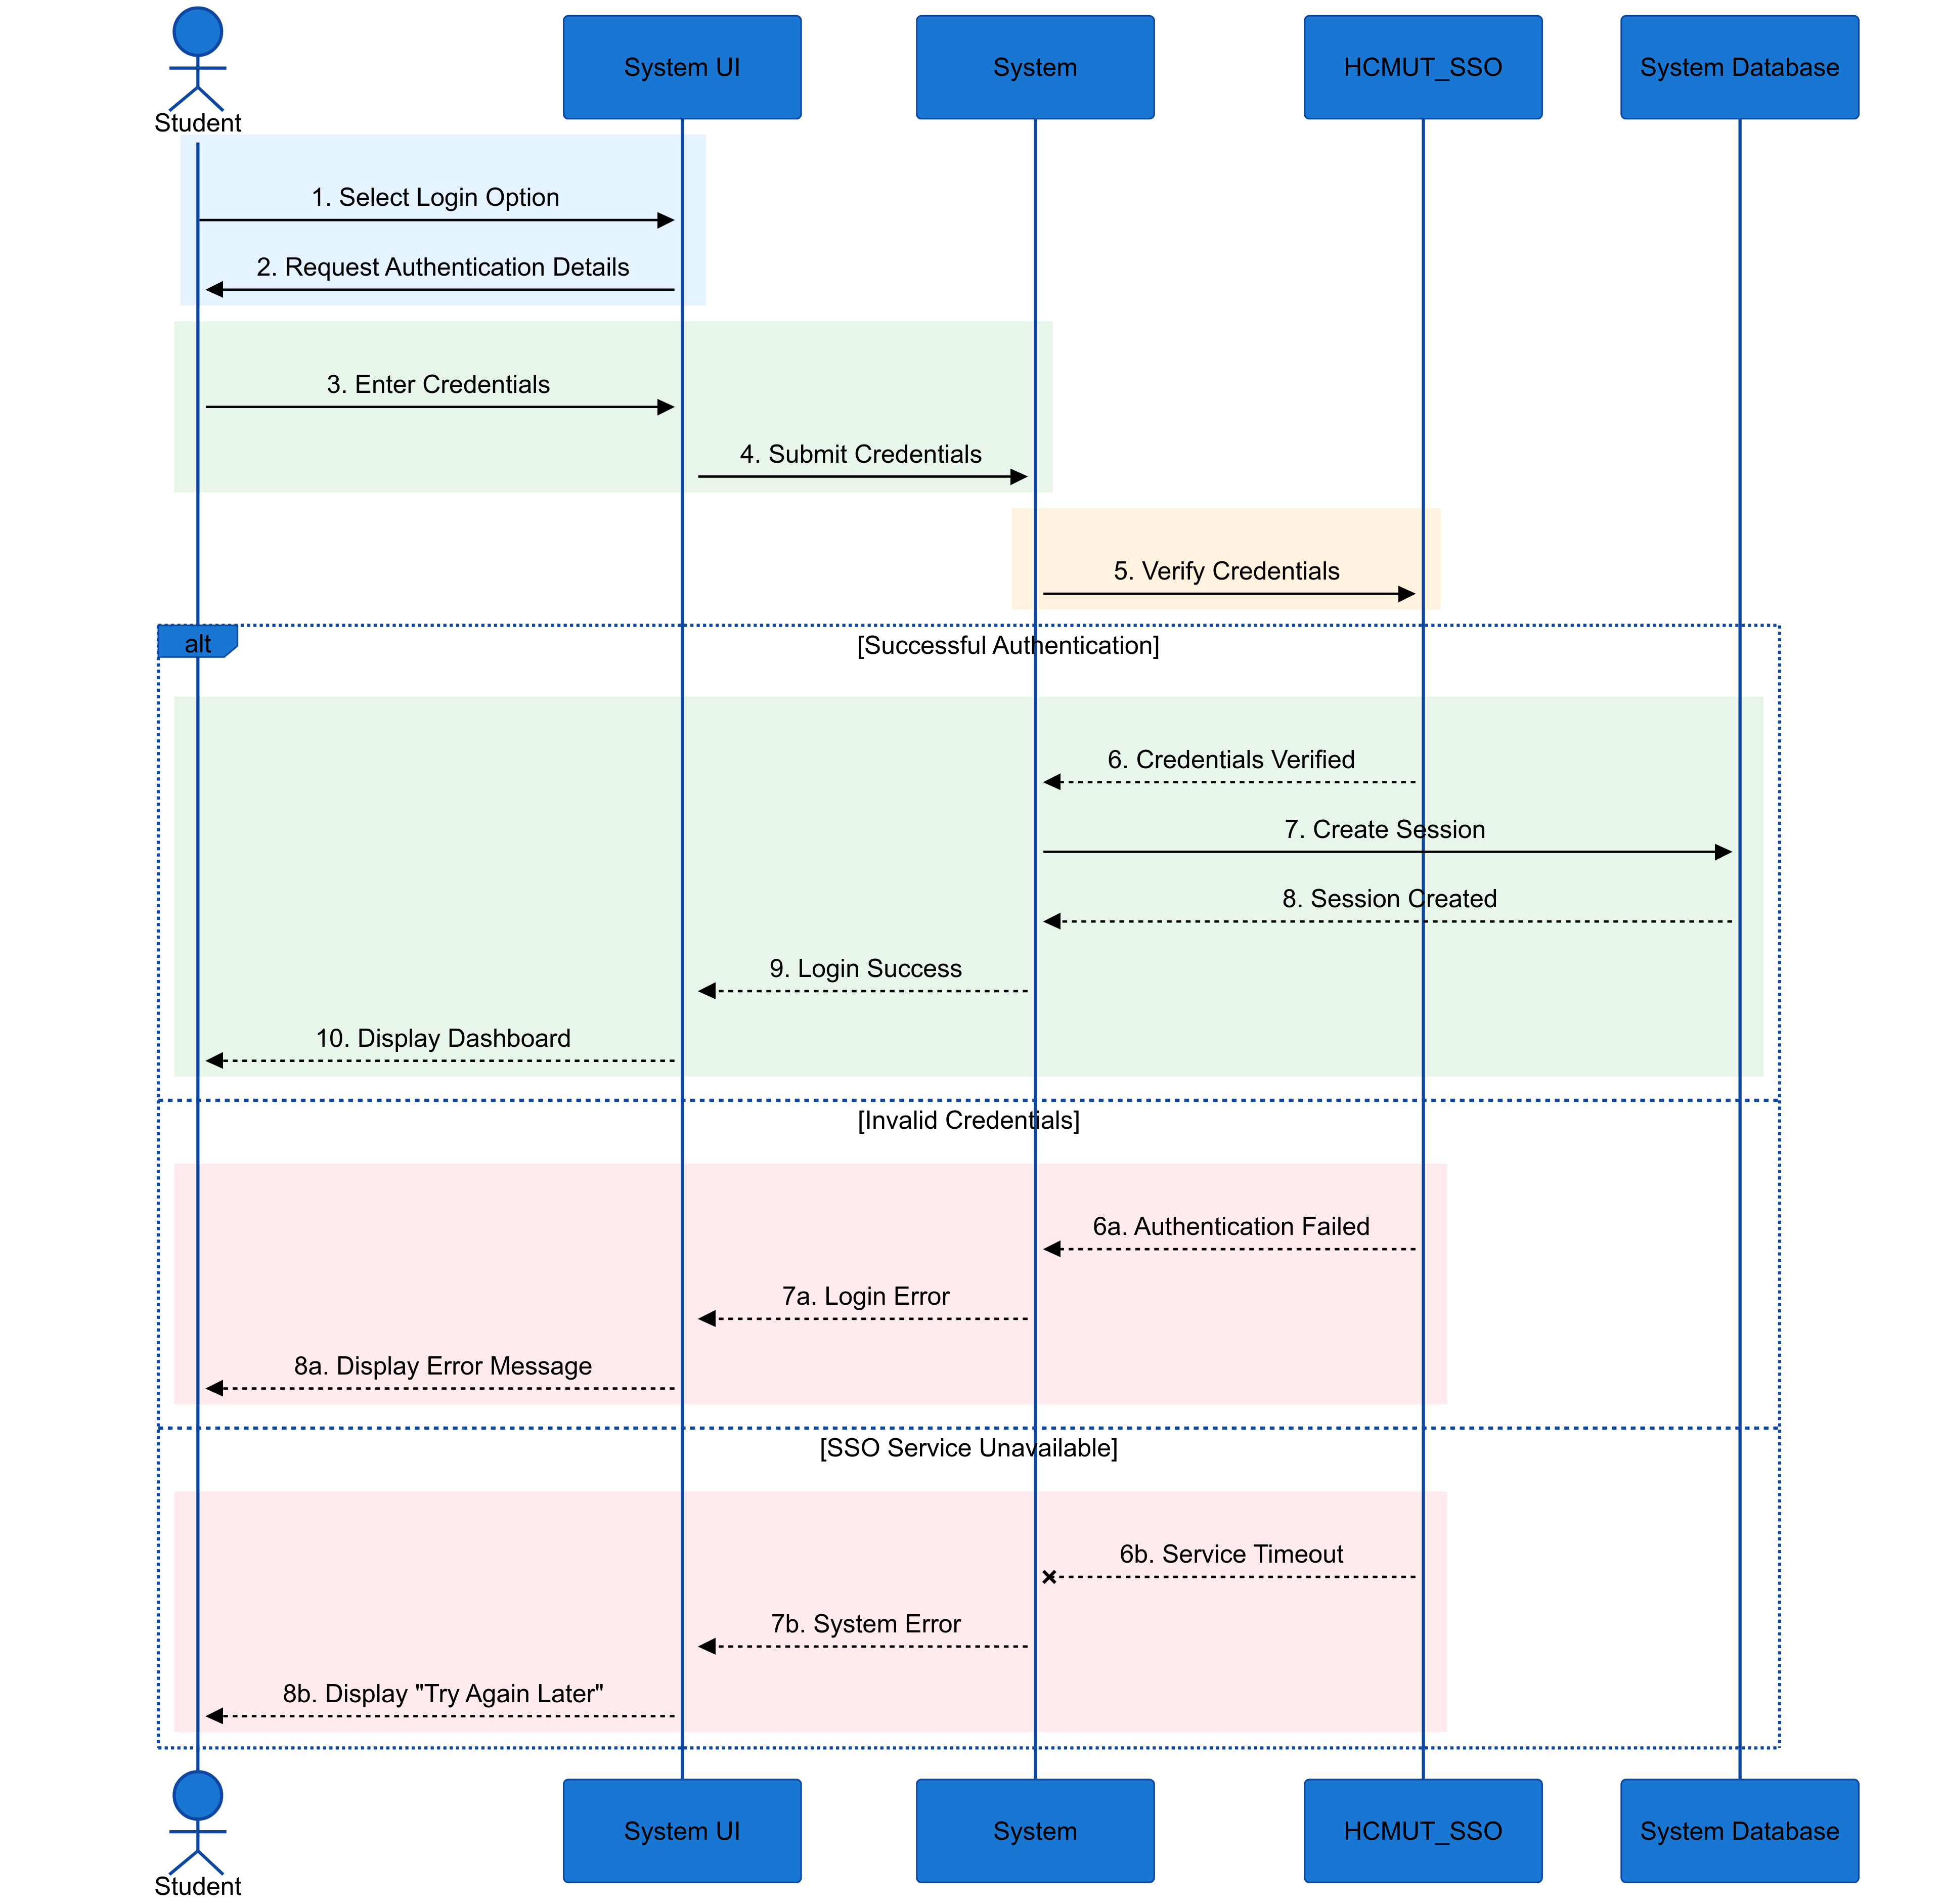
\includegraphics[width=0.85\textwidth]{images/sequence_diagram/Login.png}
    \caption{UseCase - Login}
    \label{fig:login}
\end{figure}


This sequence diagram describes the "Login" use case, where a student logs into a system via a single sign-on (SSO) service. The process starts when the student selects the login option on the system UI, prompting the system to request authentication details. The student enters their credentials, which are submitted to the SSO (HCMUT$\_$SSO) for verification.

If the credentials are correct, the SSO service verifies them, initiates a session creation request, and once the session is created, returns a success message to the system. The system then displays the main dashboard, indicating a successful login.

If the credentials are invalid, the SSO service responds with an authentication failure, prompting the system to display an error message indicating incorrect login details. Alternatively, if the SSO service is unavailable (e.g., due to a timeout), the system displays a "Try Again Later" message, informing the student of the temporary issue. This diagram comprehensively outlines the login flow, covering successful login, invalid credentials, and service unavailability scenarios, ensuring that the student receives appropriate feedback in each case.

\subsection{Usecase Doc Upload}

\begin{figure}[H]
    \centering
    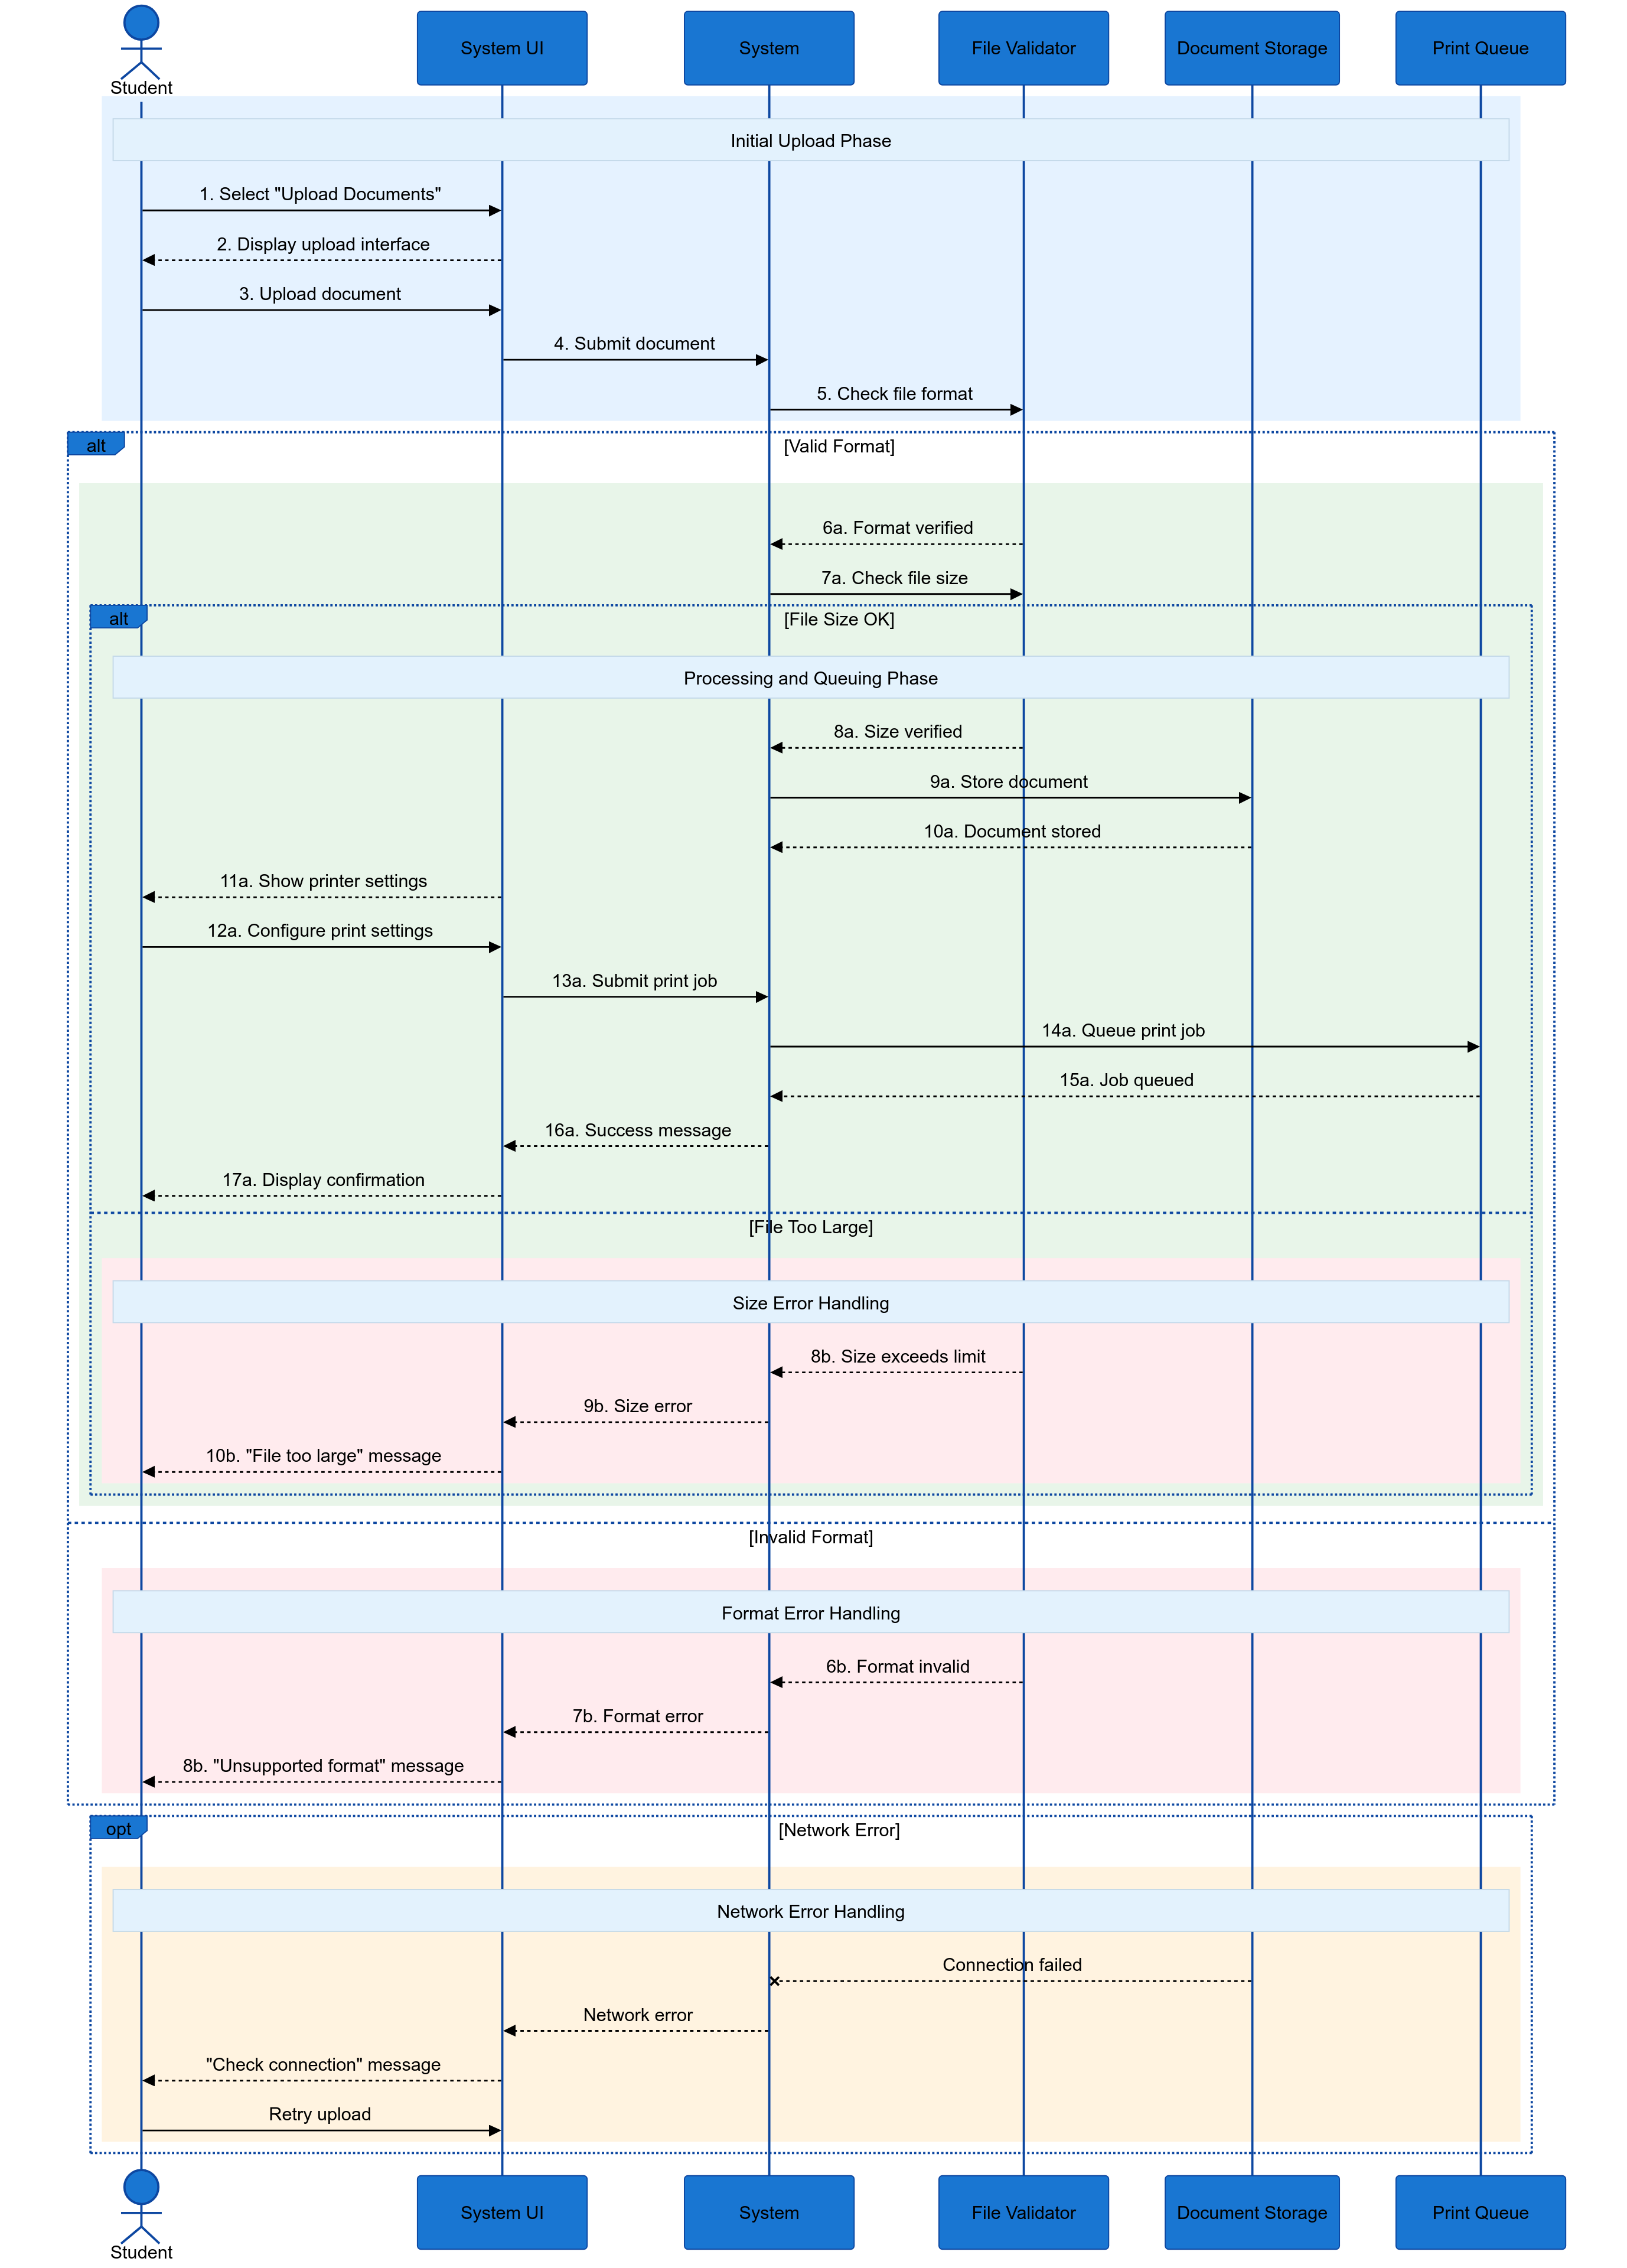
\includegraphics[width=0.9\textwidth]{images/sequence_diagram/Upload Doc.png}
    \caption{UseCase - Doc Upload}
    \label{fig:upload_doc}
\end{figure}

The diagram illustrates the "Upload Document" process, where a student begins by selecting "Upload Documents" on the UI. The student uploads a document, which is submitted to the file validator. If both the format and size are acceptable, the document is stored in the document storage system. The system then prompts the student with printer settings, allowing them to configure print options before submitting the print job. Once submitted, the document is queued, a success message is displayed to the student. If the file format or size is invalid, appropriate error messages ("Unsupported format" or "File too large") are displayed, notifying the student of the issue. In case of a network error, a "Check connection" message is shown.


% \begin{figure}[H]
%     \centering
%     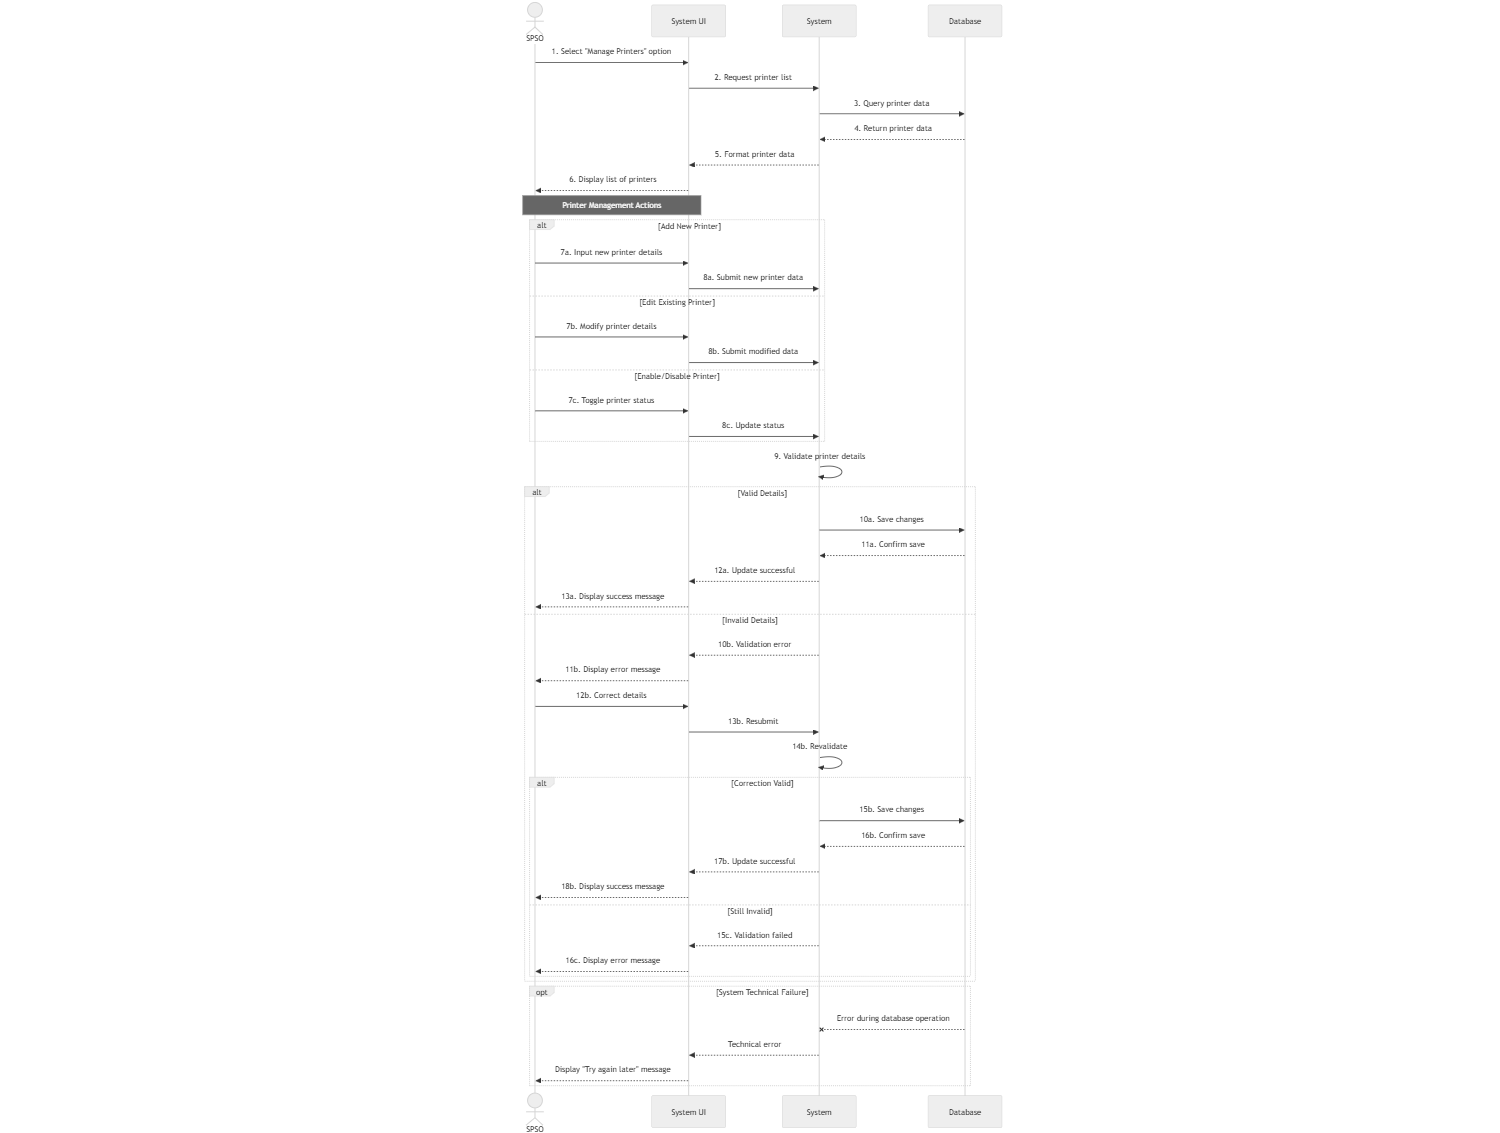
\includegraphics[width = 5in]{UseCase - Manage Printer.png}
%     \caption{UseCase - Manage Printer}
% \end{figure}

\subsection{Usecase Manage Printer}

\begin{figure}[H]
    \centering
    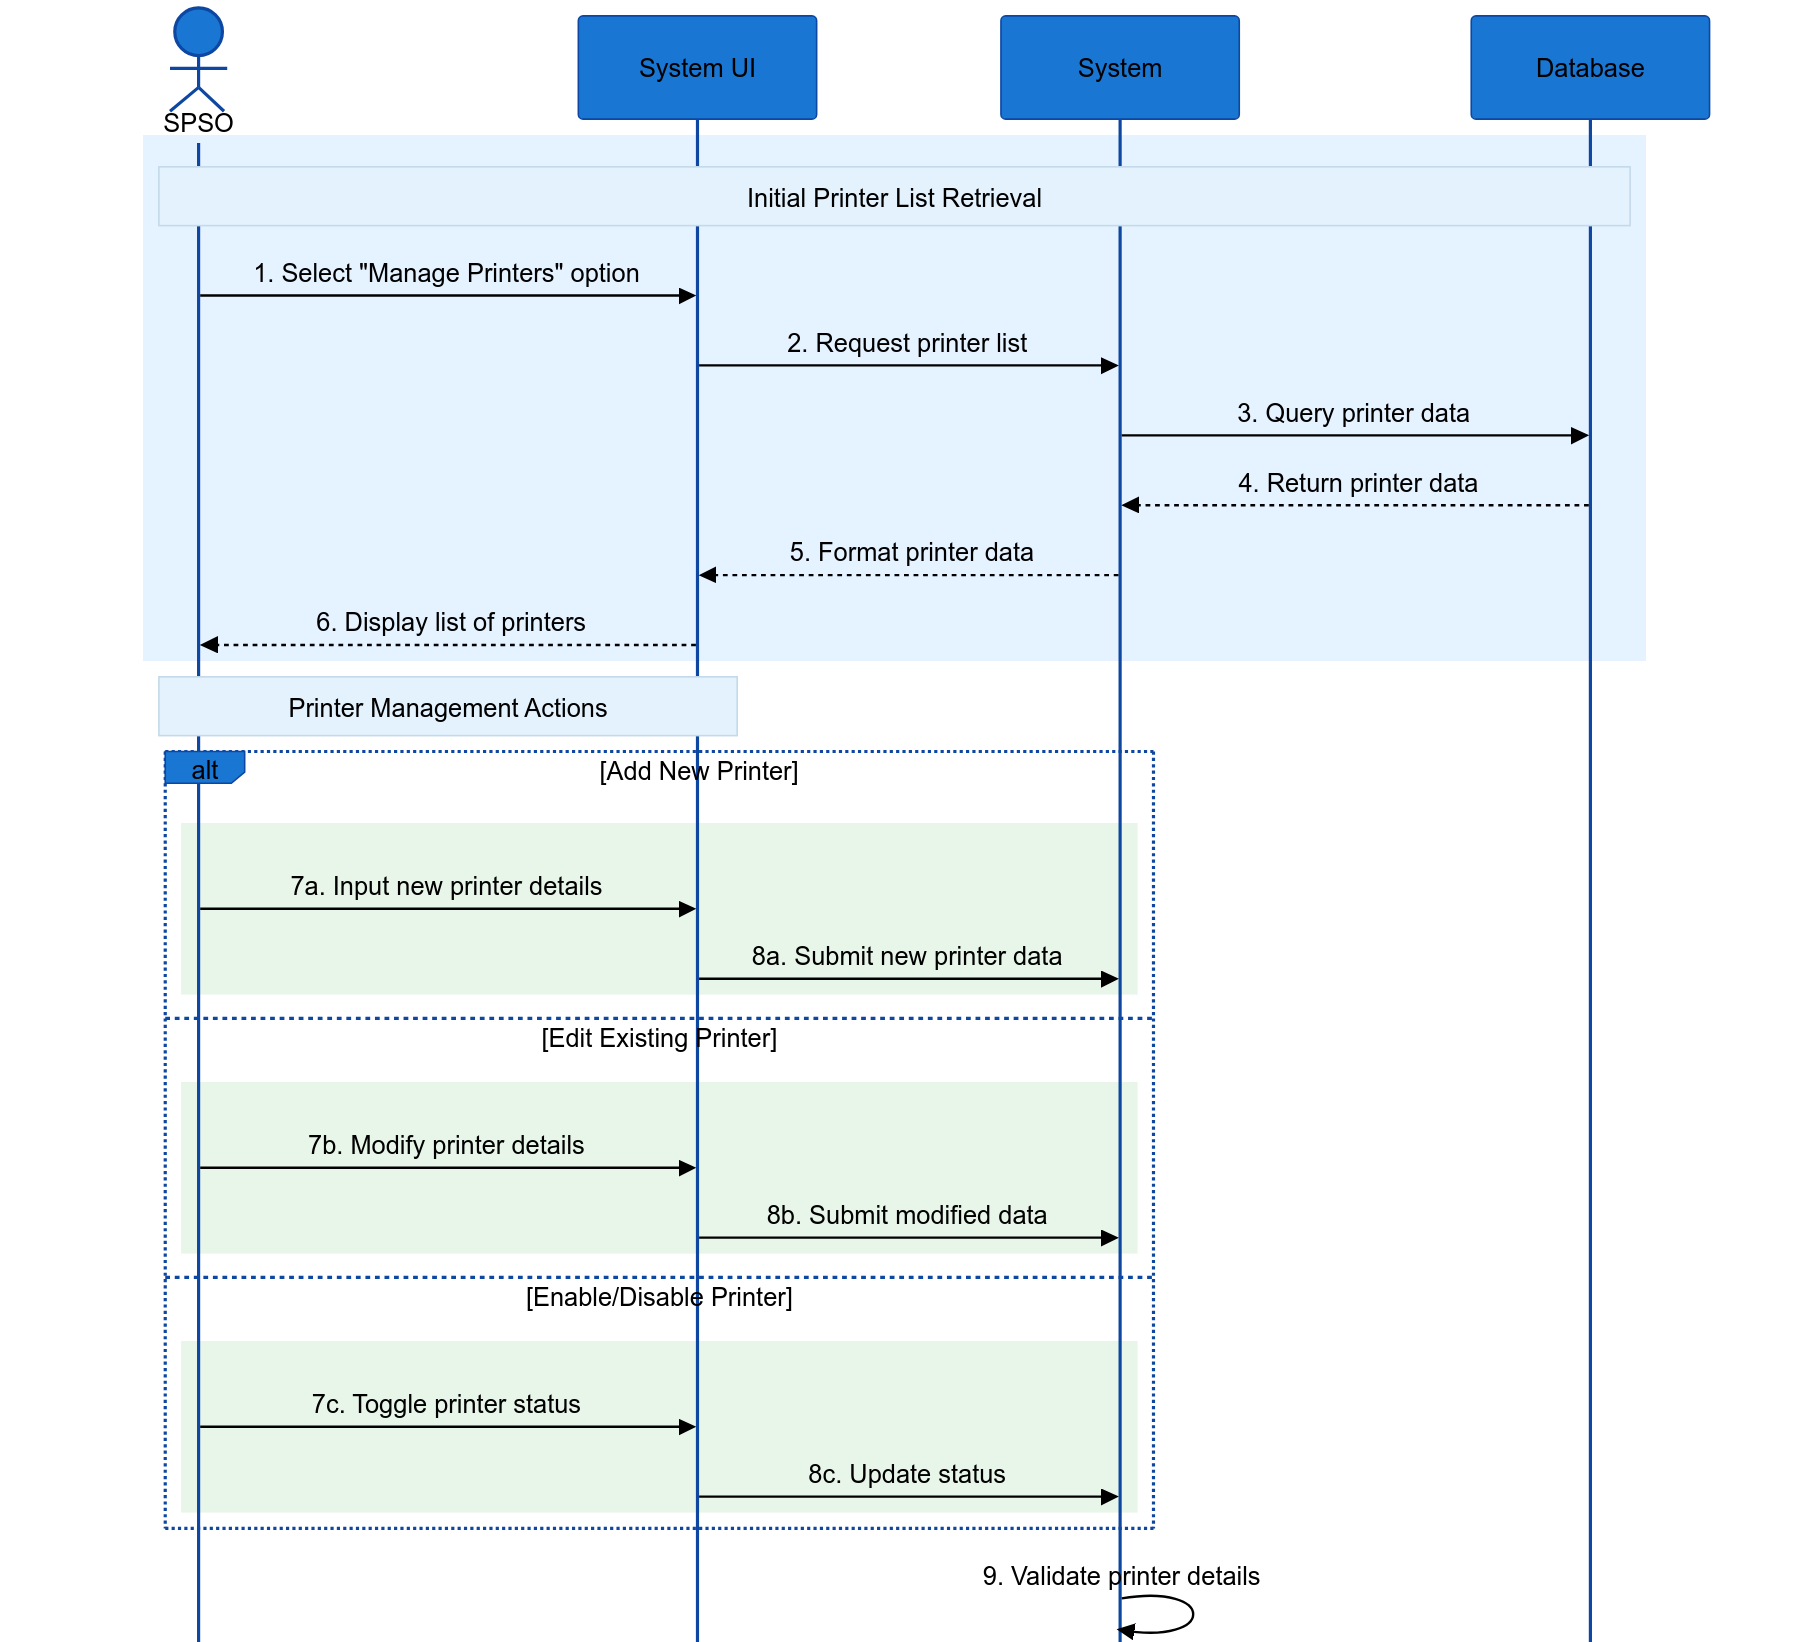
\includegraphics[width=\textwidth ]{images/sequence_diagram/Manage Printers_1.png}
    \label{fig:manage_printer}
\end{figure}

\small \textit{*Notes}: being not fit in a single page, the diagram continues on the next page.

\normalsize

\begin{figure}[H]
    \centering
    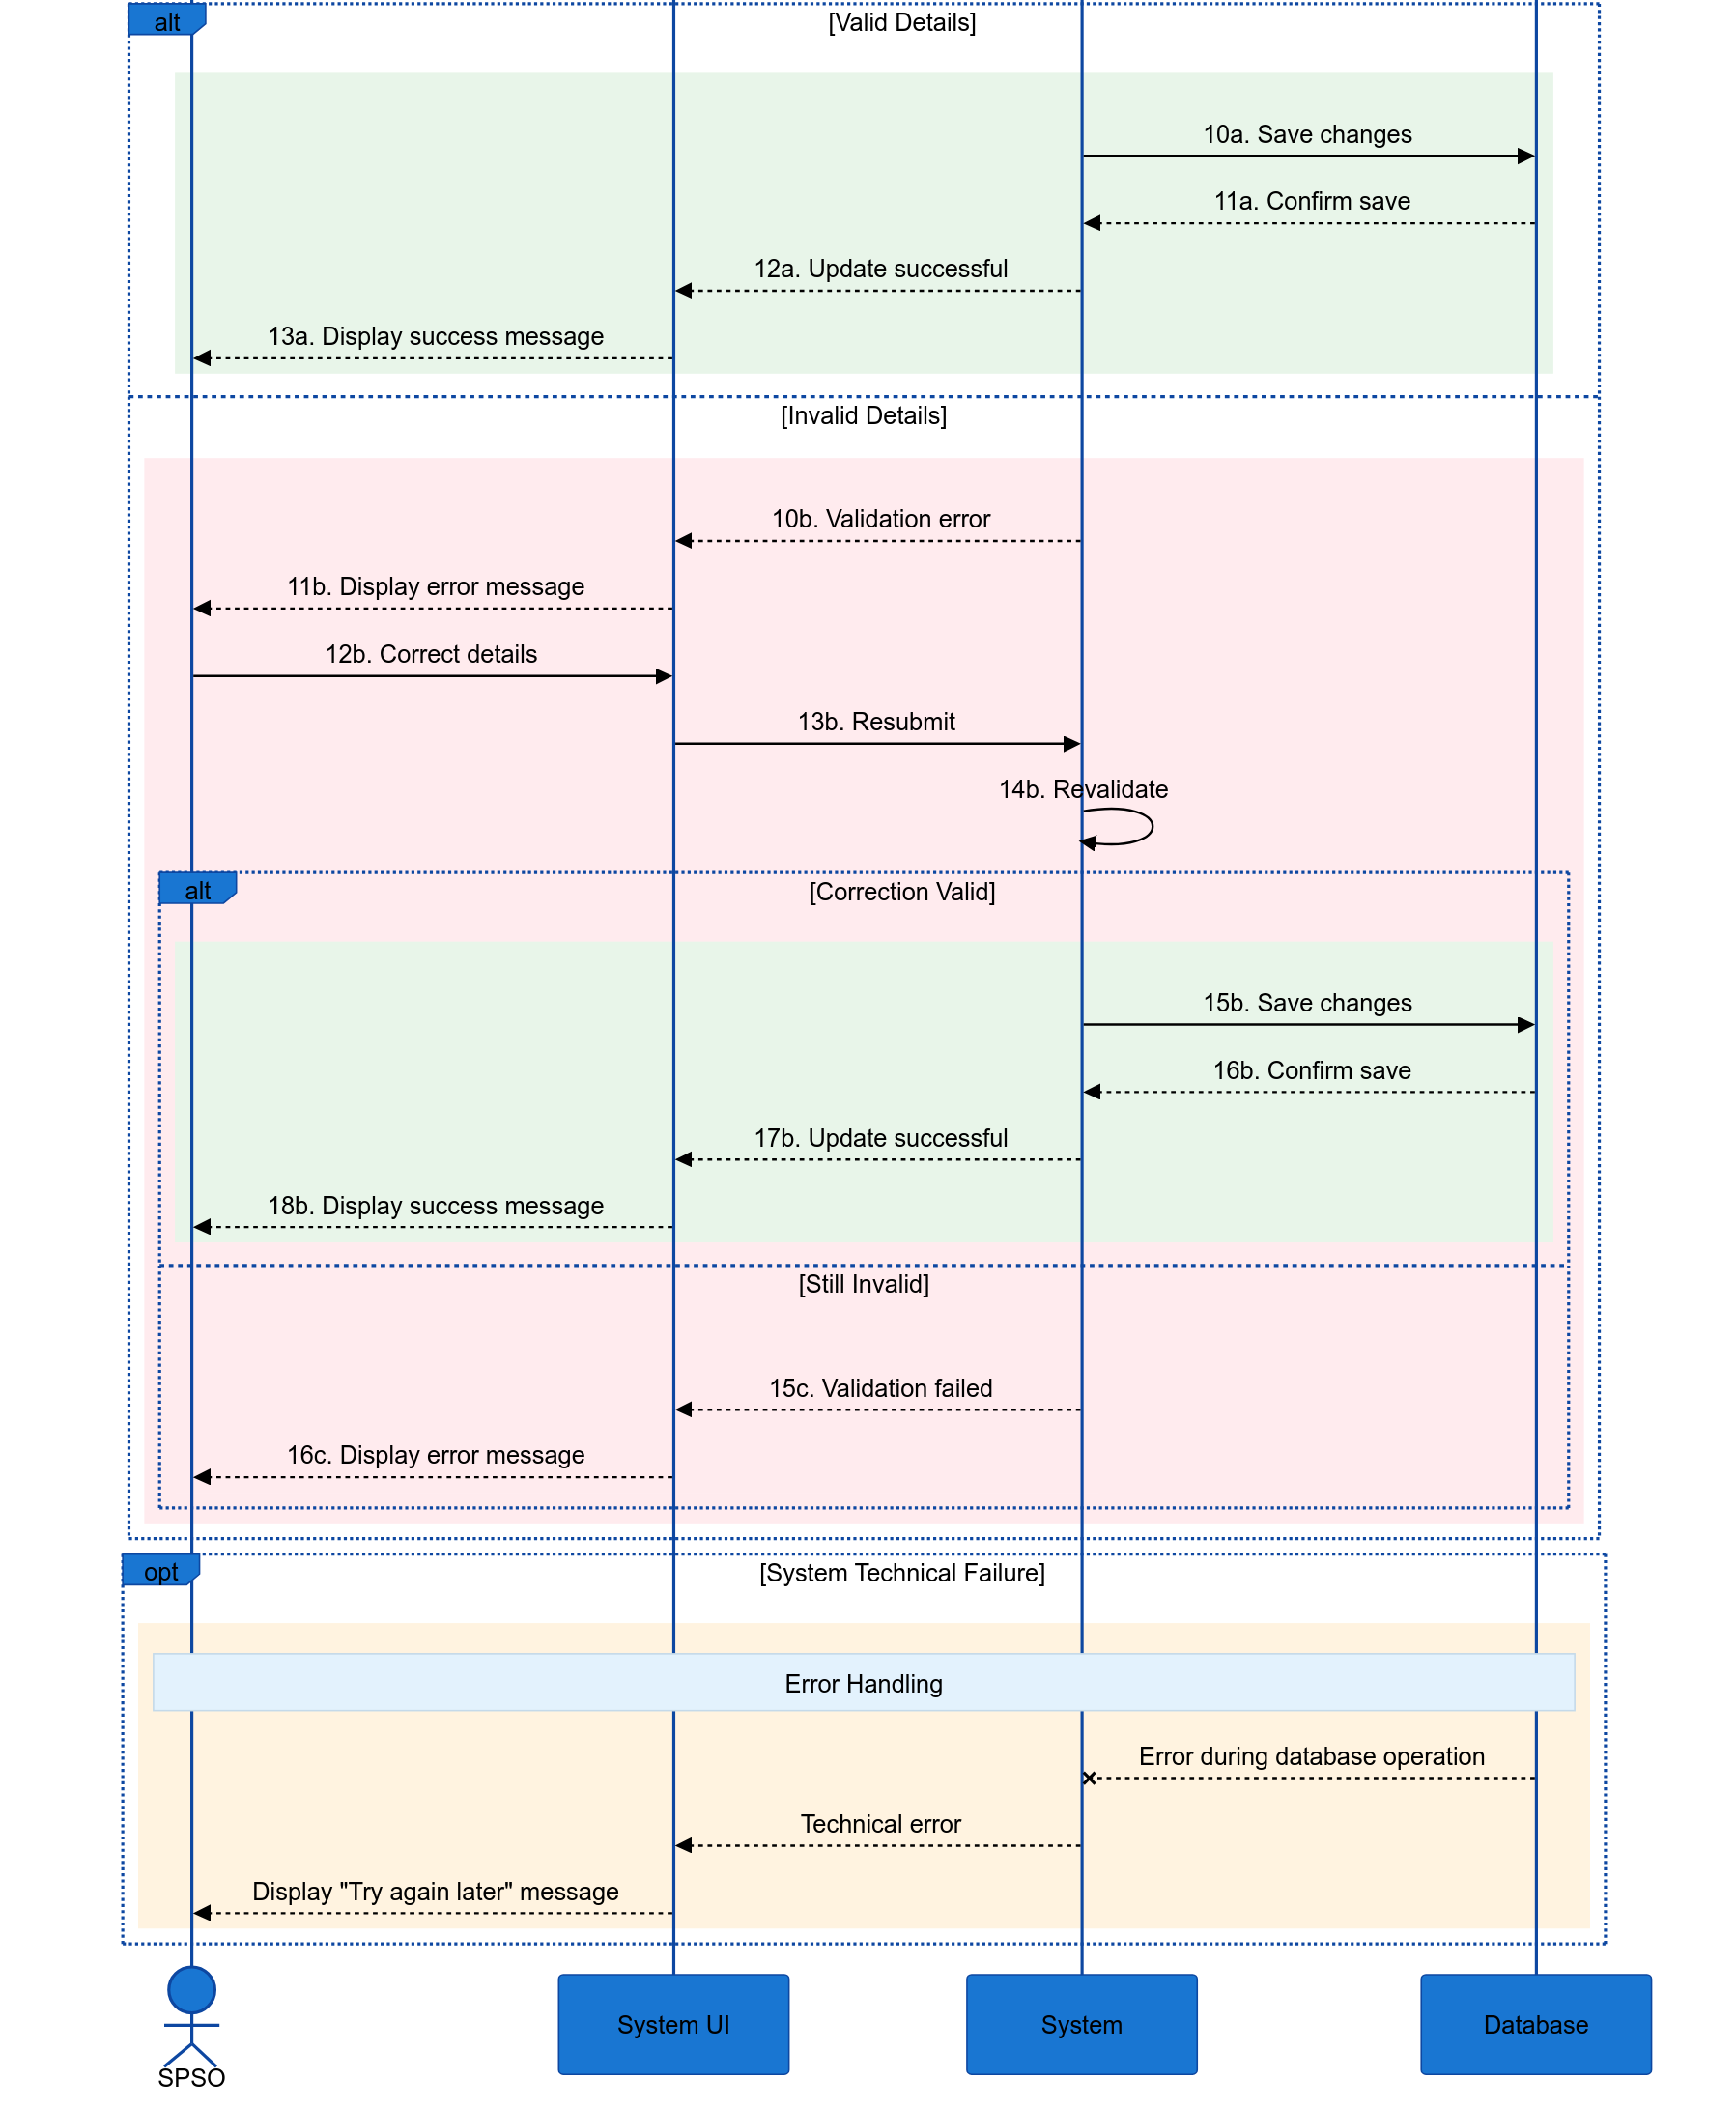
\includegraphics[width=0.9\textwidth ]{images/sequence_diagram/Manage Printers_2.png}
    \caption{UseCase - Manage Printer}
    \label{fig:manage_printer}
\end{figure}

The diagram details the "Manage Printers" usecase, where an SPSO manages printer settings in a system. The process starts when SPSO clicks "Manage Printers", prompting the system to request and retrieve the printer list from the database. The system then displays the list of printer management actions, which can include adding a new printer, editing an existing printer, or enabling/disabling a printer.

In the flow \textbf{Add New Printer}, the SPSO inputs new printer details, submits them, and the system validates the information before committing it to the database. 
In the flow \textbf{Edit Existing Printer}, the SPSO modifies printer details, submits the changes, and the system validates the information before saving. 
In the flow \textbf{Enable/Disable Printer}, the SPSO toggles the printer status, and the system updates this change in the database. In all flows, the system returns a success message if valid.

If any information is invalid during validation, an error message is displayed, prompting the SPSO to correct and resubmit the details. If validation fails again or if there's a technical error during database operations, the system displays relevant error messages ("Try again later") to inform the SPSO of the issue. This sequence covers various printer management operations, ensuring error handling, validation, and system feedback for a seamless user experience.


\subsection{Usecase Buy More Page}

\begin{figure}[H]
    \centering
    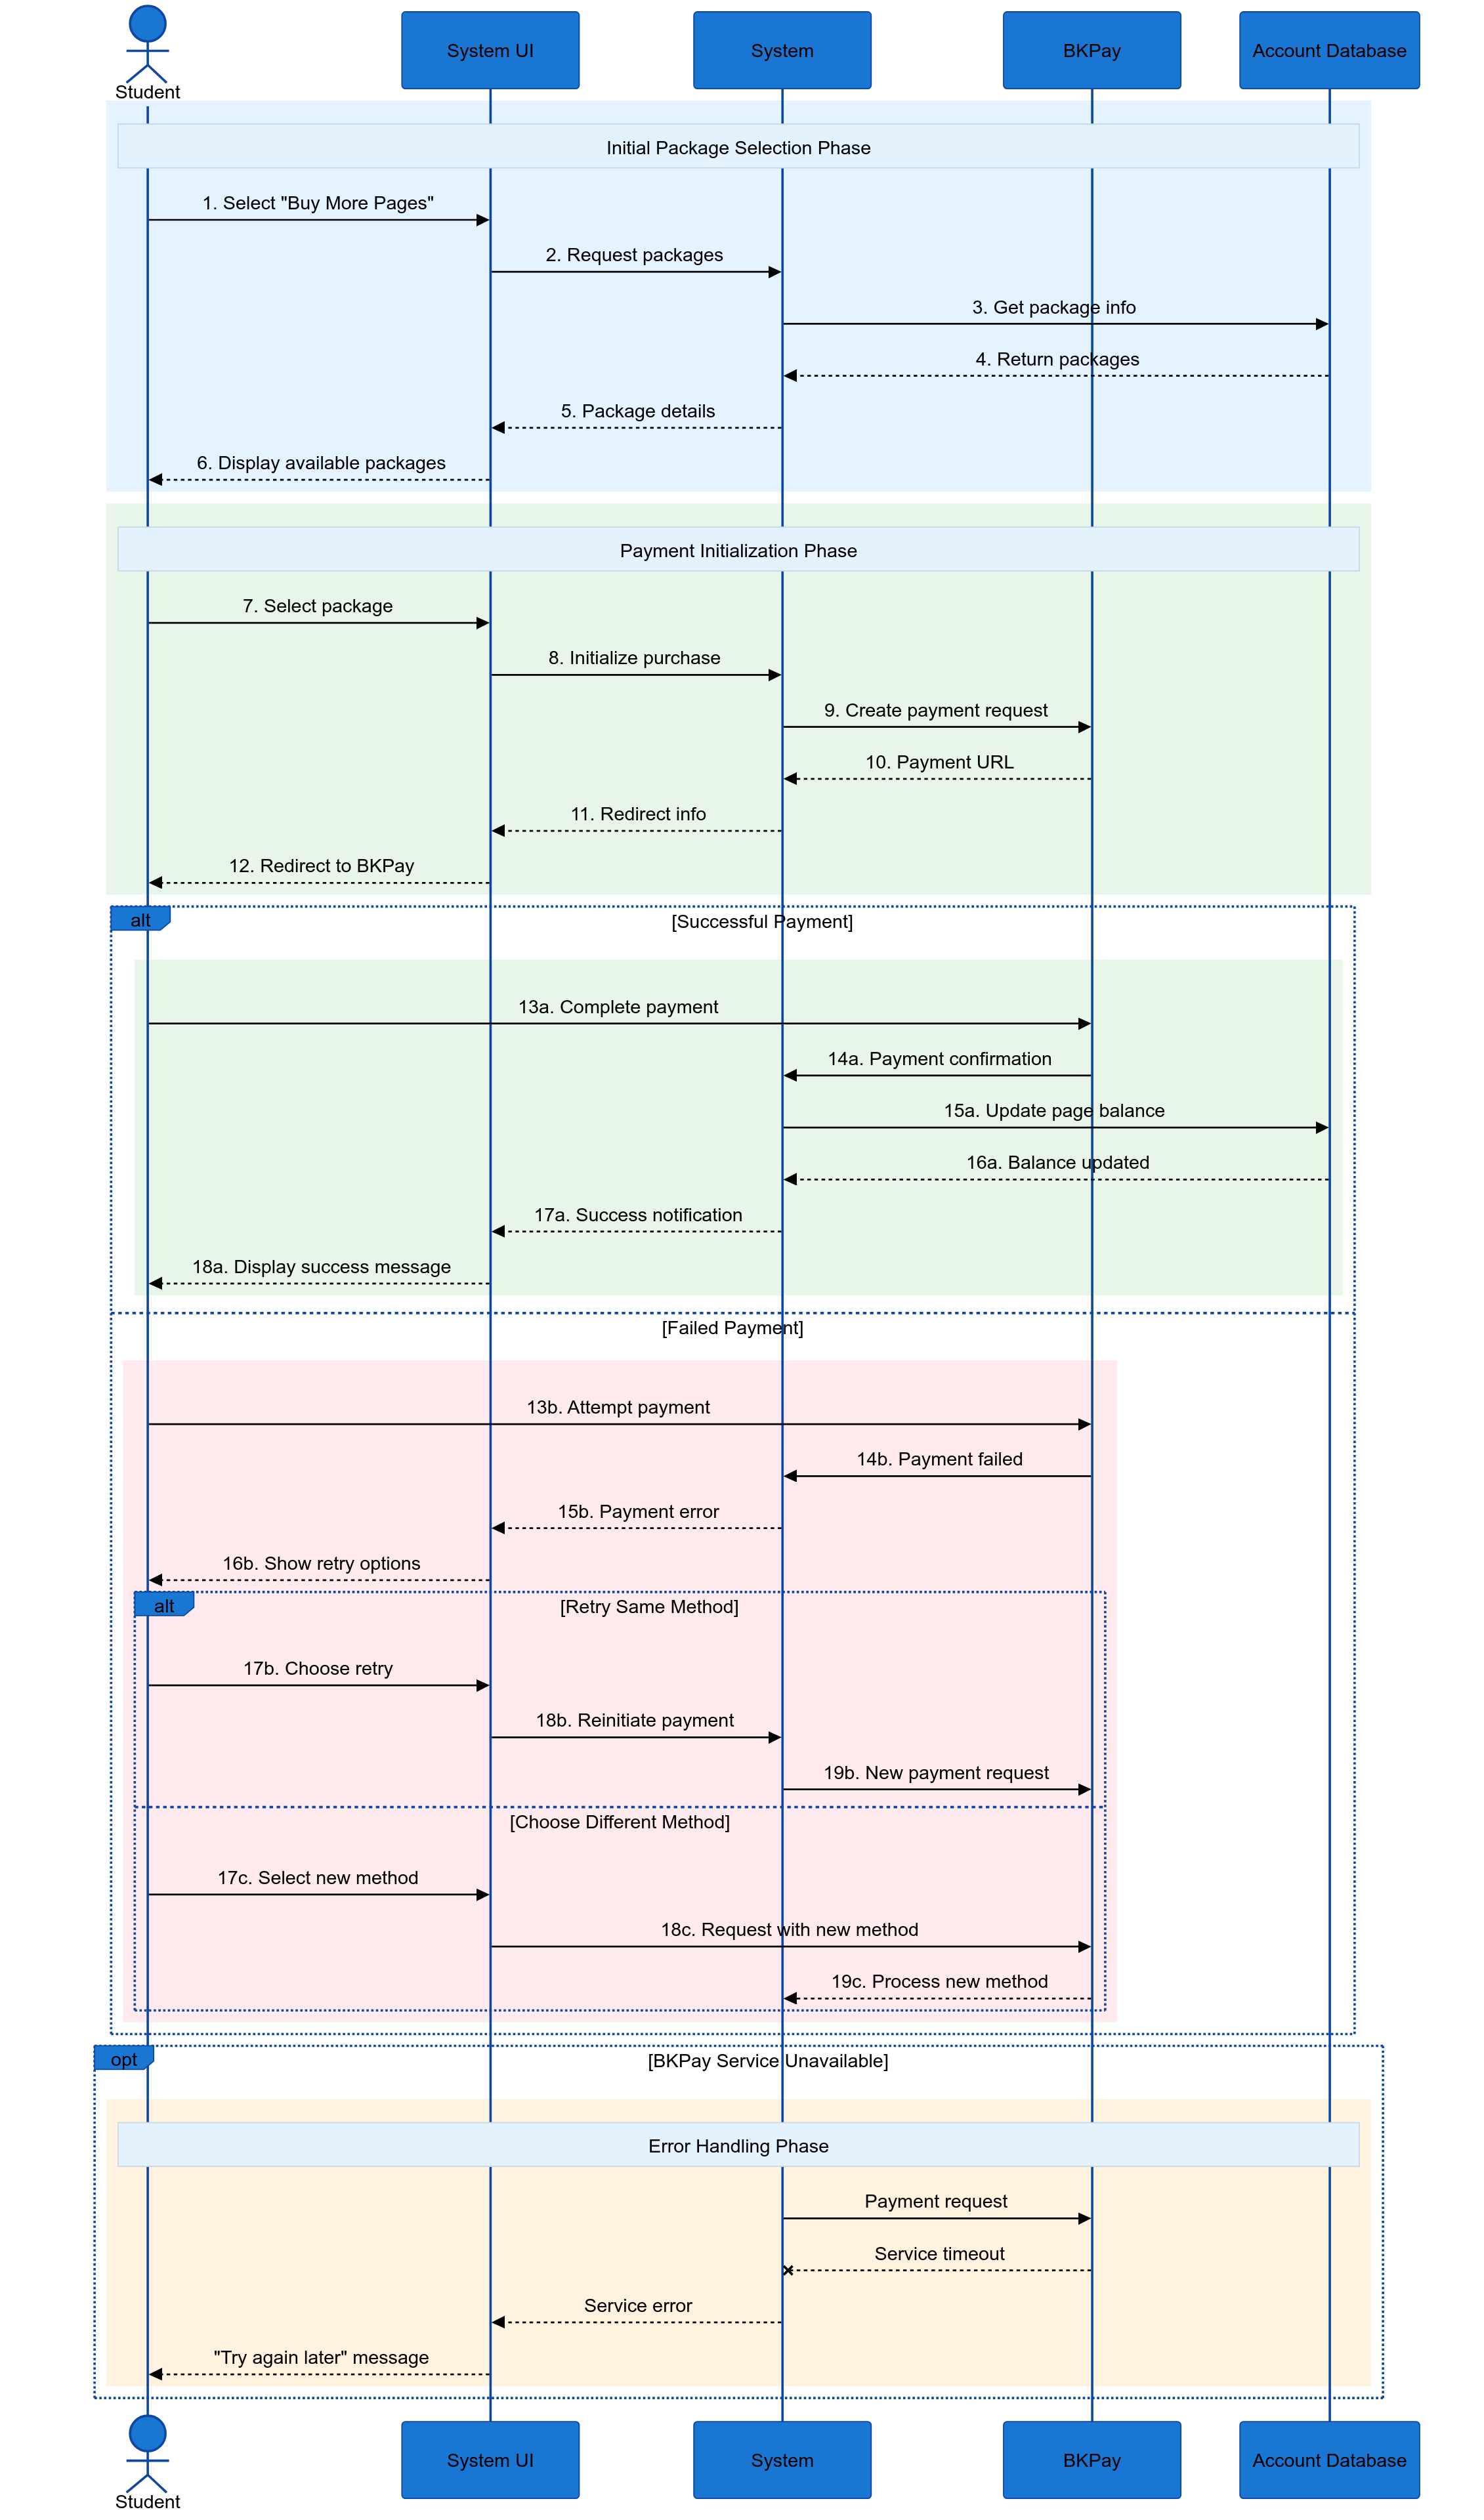
\includegraphics[width=0.8\textwidth]{images/sequence_diagram/Buy More Pages.png}
    \caption{UseCase - Buy More Page}
    \label{fig:buy_more_page}
\end{figure}

This sequence diagram outlines the "Buy More Pages" process, where a student initiates a request by selecting "Buy More Pages" on the system UI. The system retrieves available packages and displays them to the student, who then selects a desired package. Upon package selection, a purchase request is sent to the payment gateway (BKPay), which initializes the payment process and redirects the user for payment. If the payment is successful, a confirmation is sent to the system, which then updates the student's page balance in the account database and displays a success message. In case of payment failure, the system provides retry options, allowing the student to either retry with the same method or choose a different payment method. If the payment gateway service is temporarily unavailable, a "Service error" message is displayed, and the student is advised to "try again later." This diagram ensures a comprehensive understanding of the "Buy More Pages" process, covering successful transactions, error handling, and retry options to enhance user experience.

\subsection{Usecase View Printing Logs}

\begin{figure}[H]
    \centering
    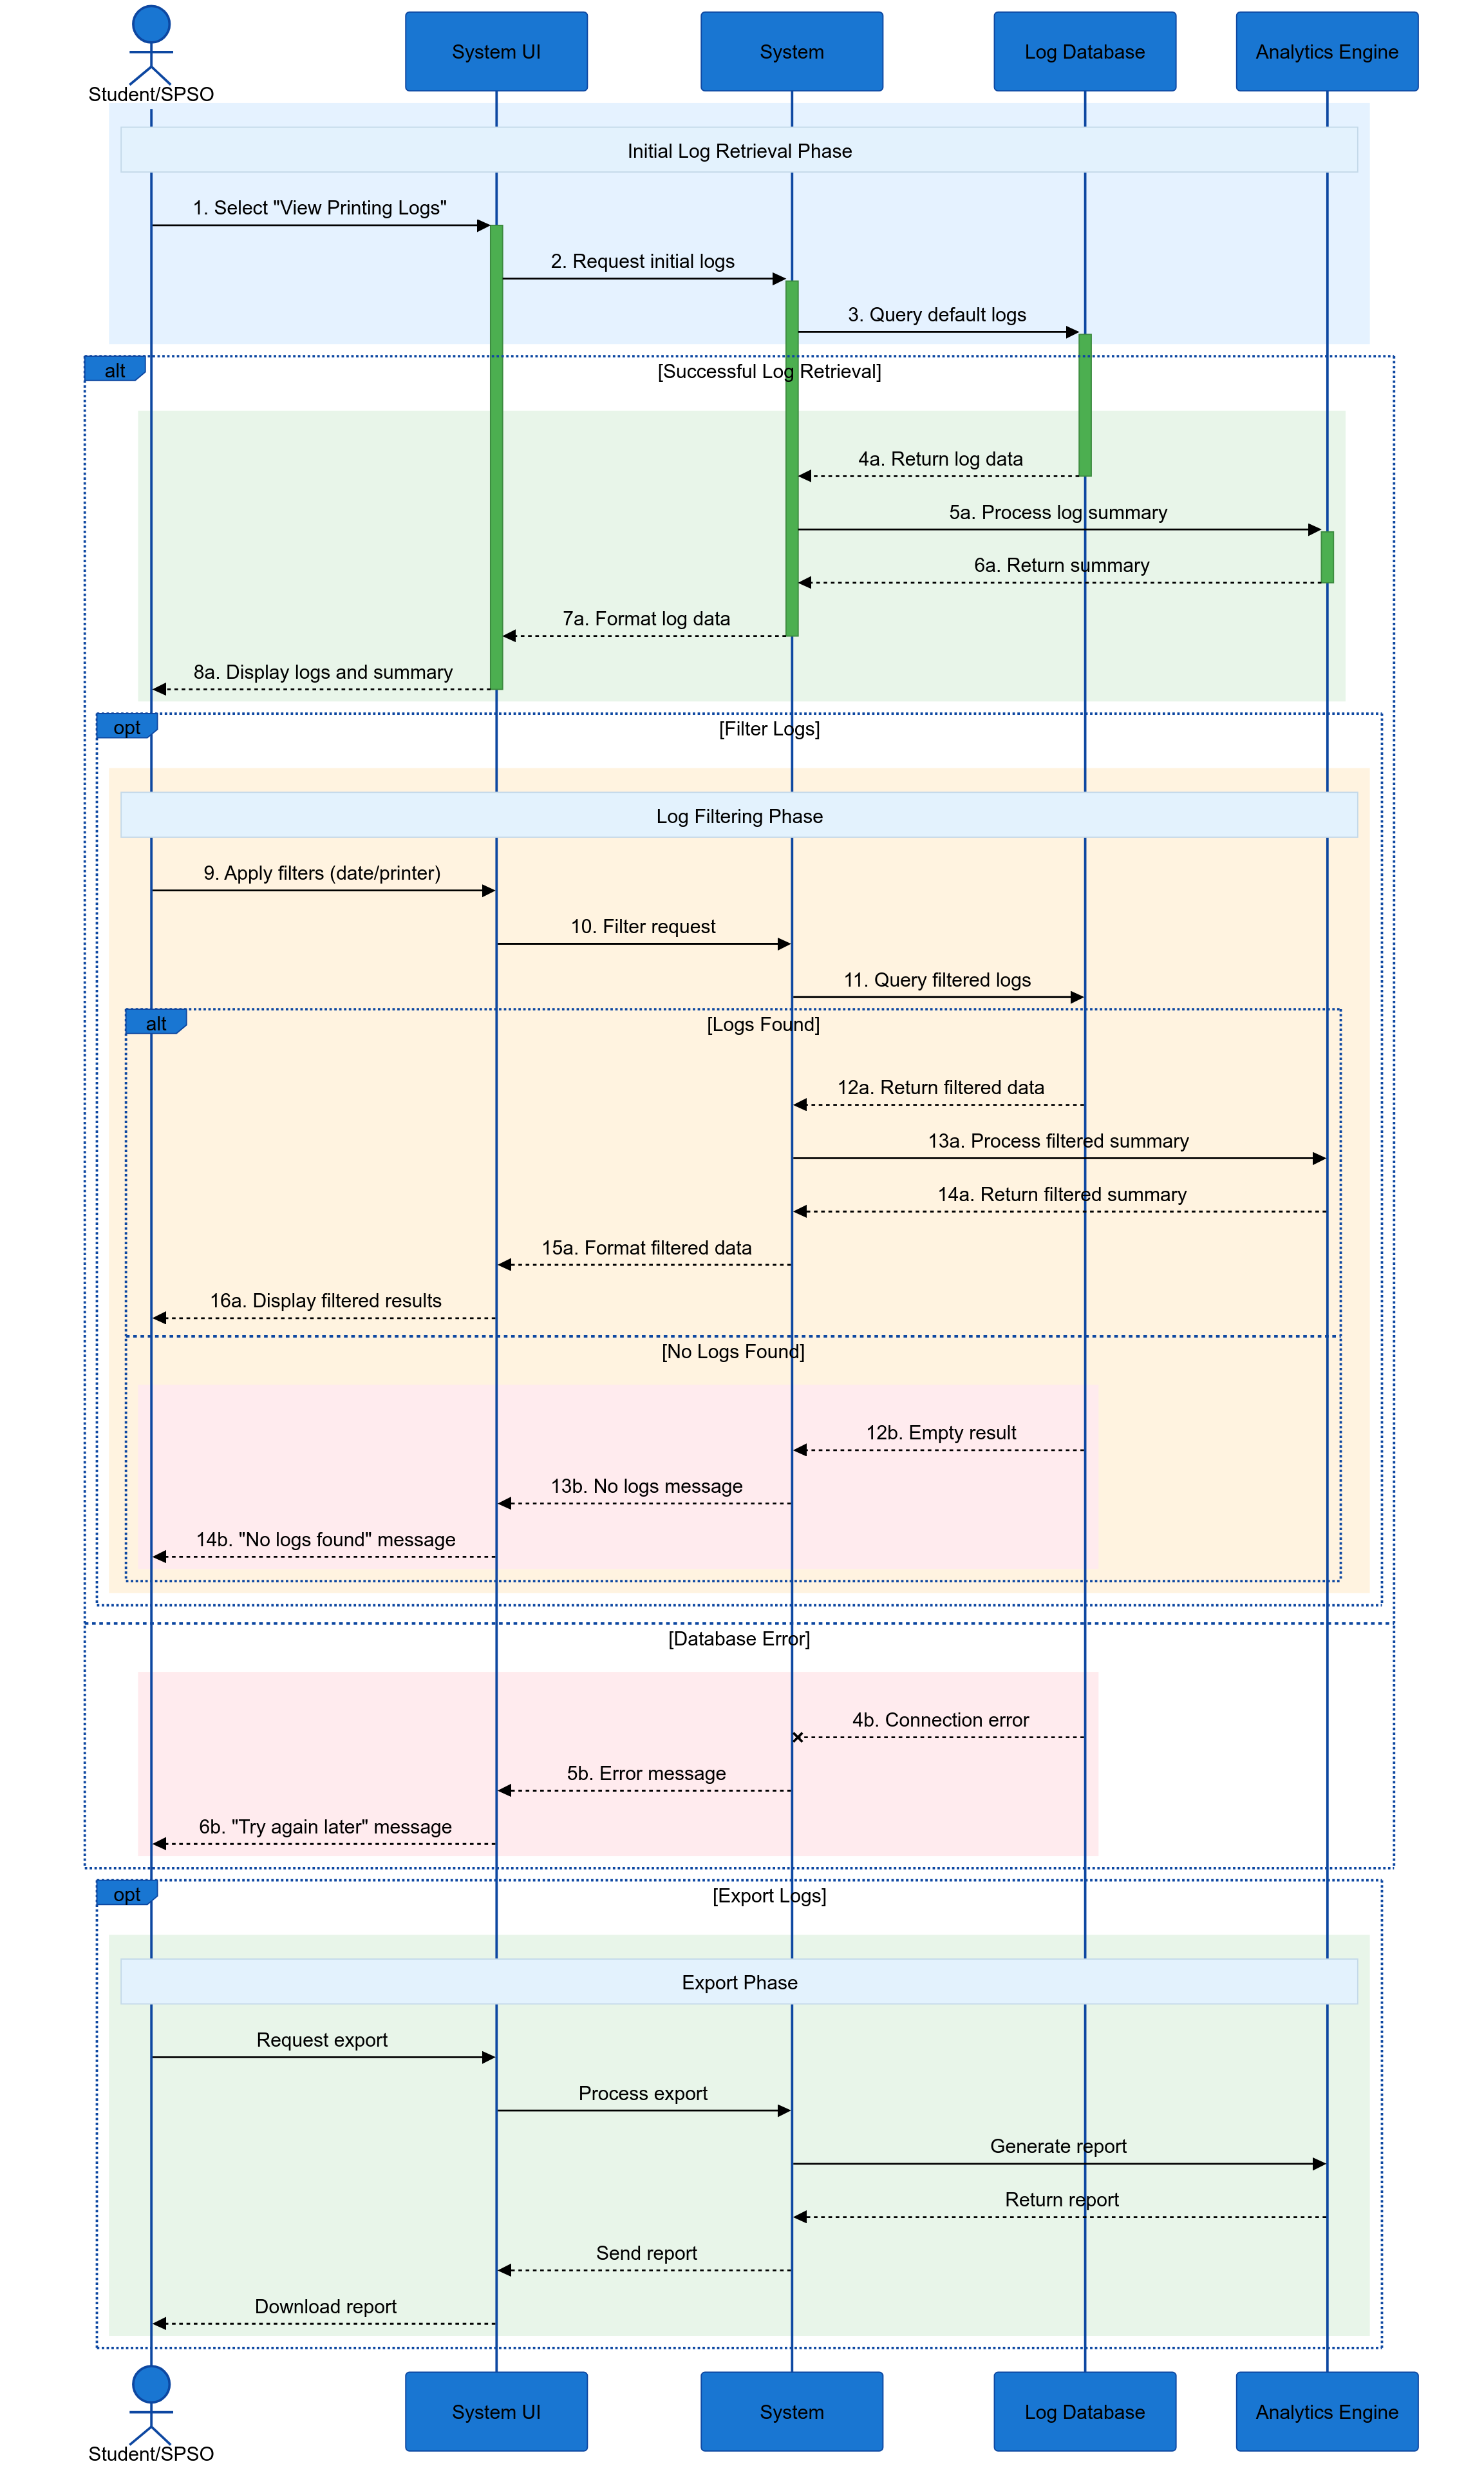
\includegraphics[width=0.85\textwidth]{sequence_diagram/View Printing Logs.png}
    \caption{UseCase - View Priting Logs}
    \label{fig:view_printing_logs}
    
\end{figure}

This diagram (Figure \ref{fig:view_printing_logs}) represents a use case for viewing printing logs in a system. It begins with a "Student/SPSO" selecting the "View Printing Logs" option. The system then initiates a request to retrieve initial logs, querying the default logs from the log database. If log retrieval is successful, the log data is returned, and a log summary is processed by the analytics engine, followed by the formatted log data and summary being displayed. The user has the option to apply filters such as date or printer, which triggers another query to retrieve filtered logs. If logs are found, the system returns the filtered data and displays it; otherwise, a "No logs found" message is shown. In case of a database error, an error message is shown with a suggestion to "try again later." Additionally, the user can request to export the logs, which prompts the system to process and generate a report for download. This sequence ensures comprehensive interaction flows for log viewing, filtering, error handling, and export functionalities.

\section{Class Diagram}
\newpage
\thispagestyle{empty}
\begin{landscape} % Start landscape mode
    
    \begin{figure}[H]
        \centering
        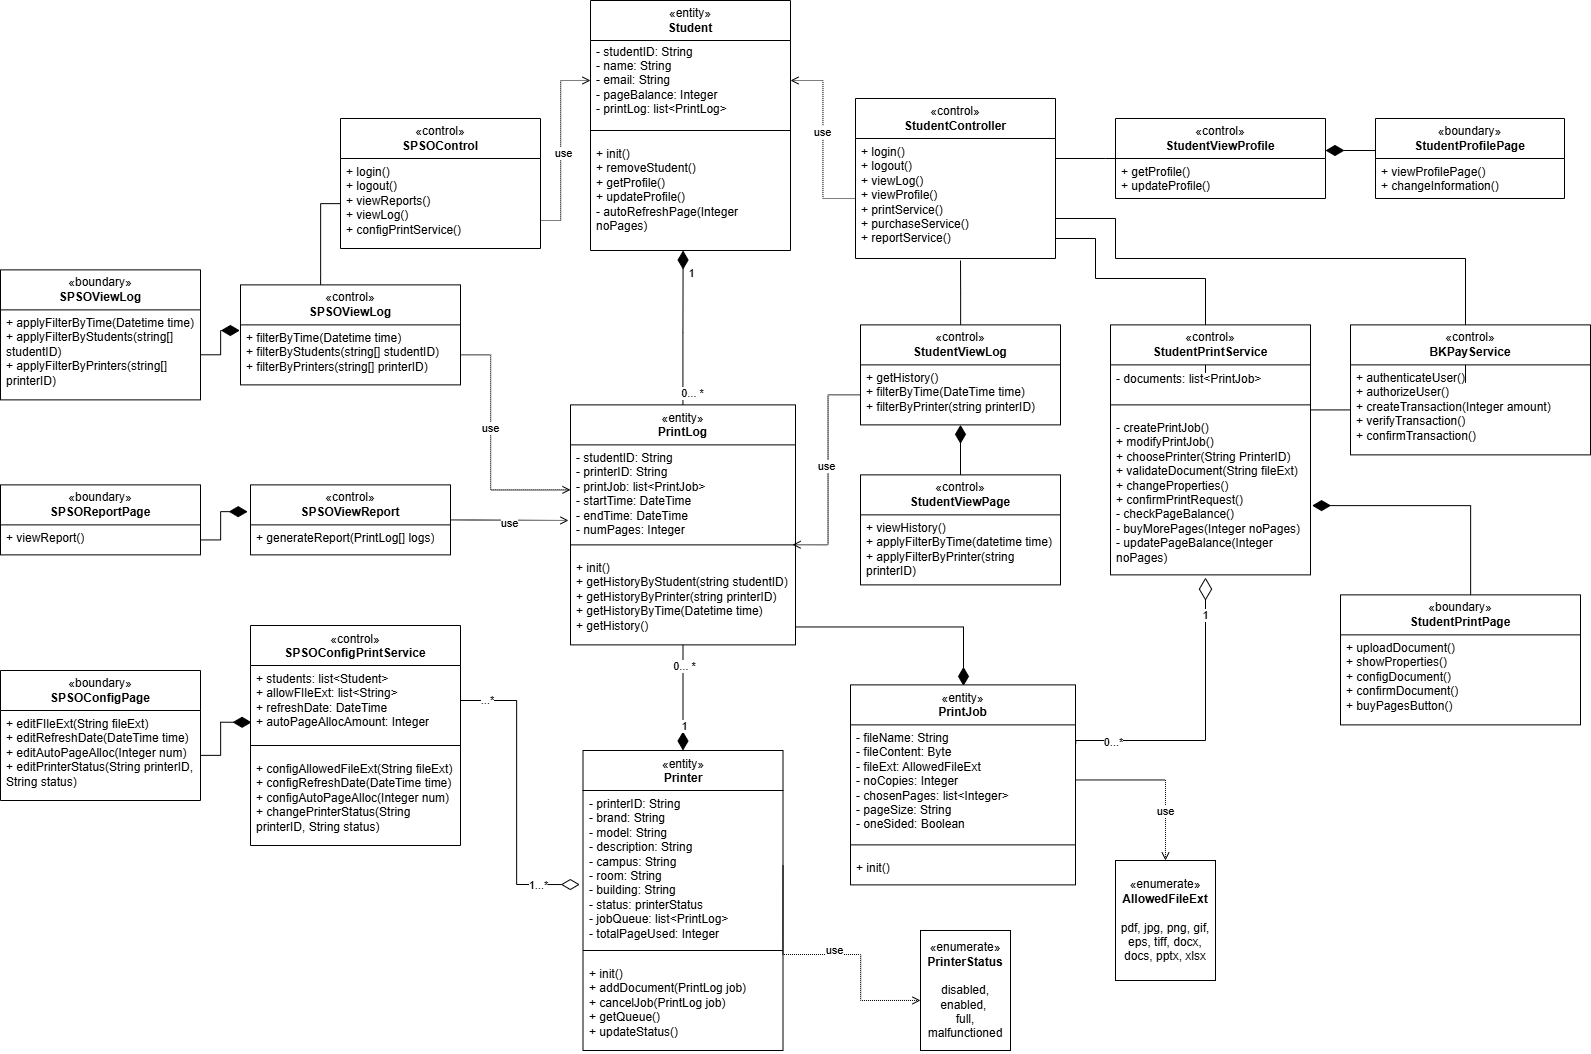
\includegraphics[width=1.3\textwidth]{class_diagram.png}
            \caption{Class Diagram}
        \label{fig:class_diagram}
    \end{figure}    
    
\end{landscape} % End landscape mode

\newpage
\section{Development MVP 1}

\begin{figure}[H]
    \centering
    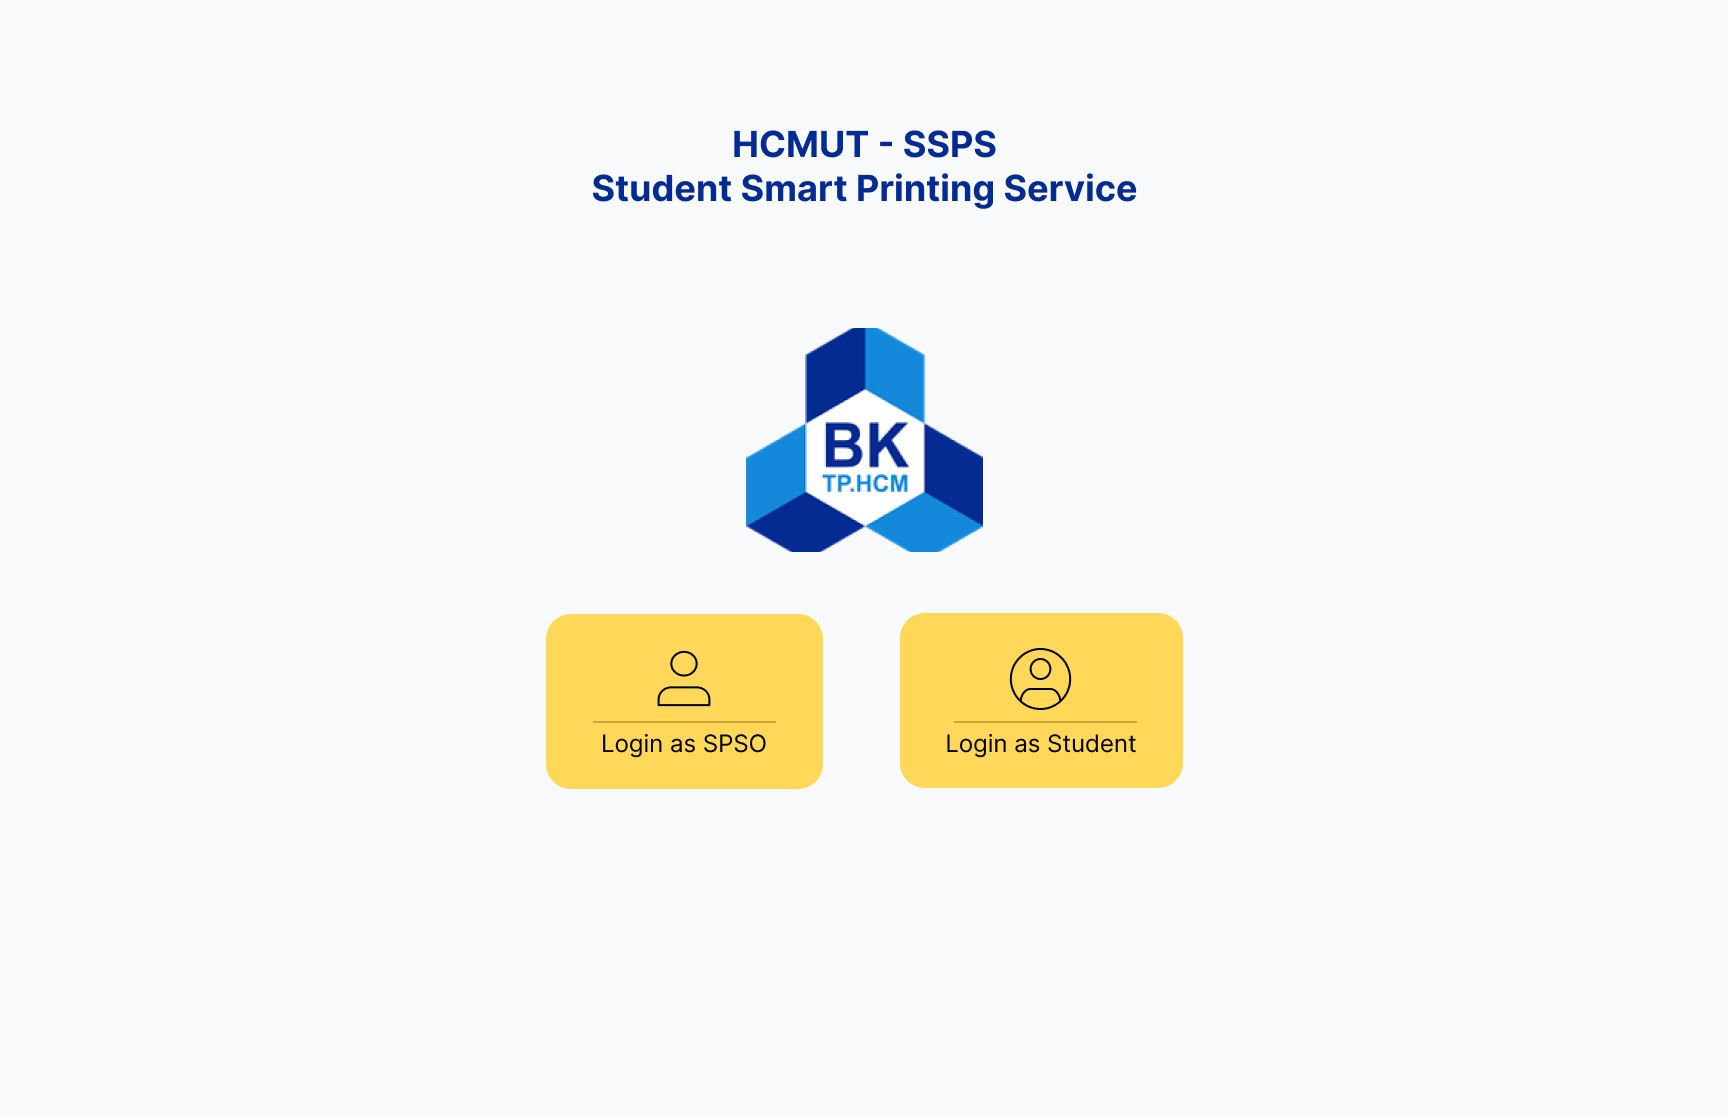
\includegraphics[width = 1\textwidth, ]{images/UI/Login Page.png}
    \caption{Login Page}
\end{figure}  

\begin{figure}[H]
    \centering
    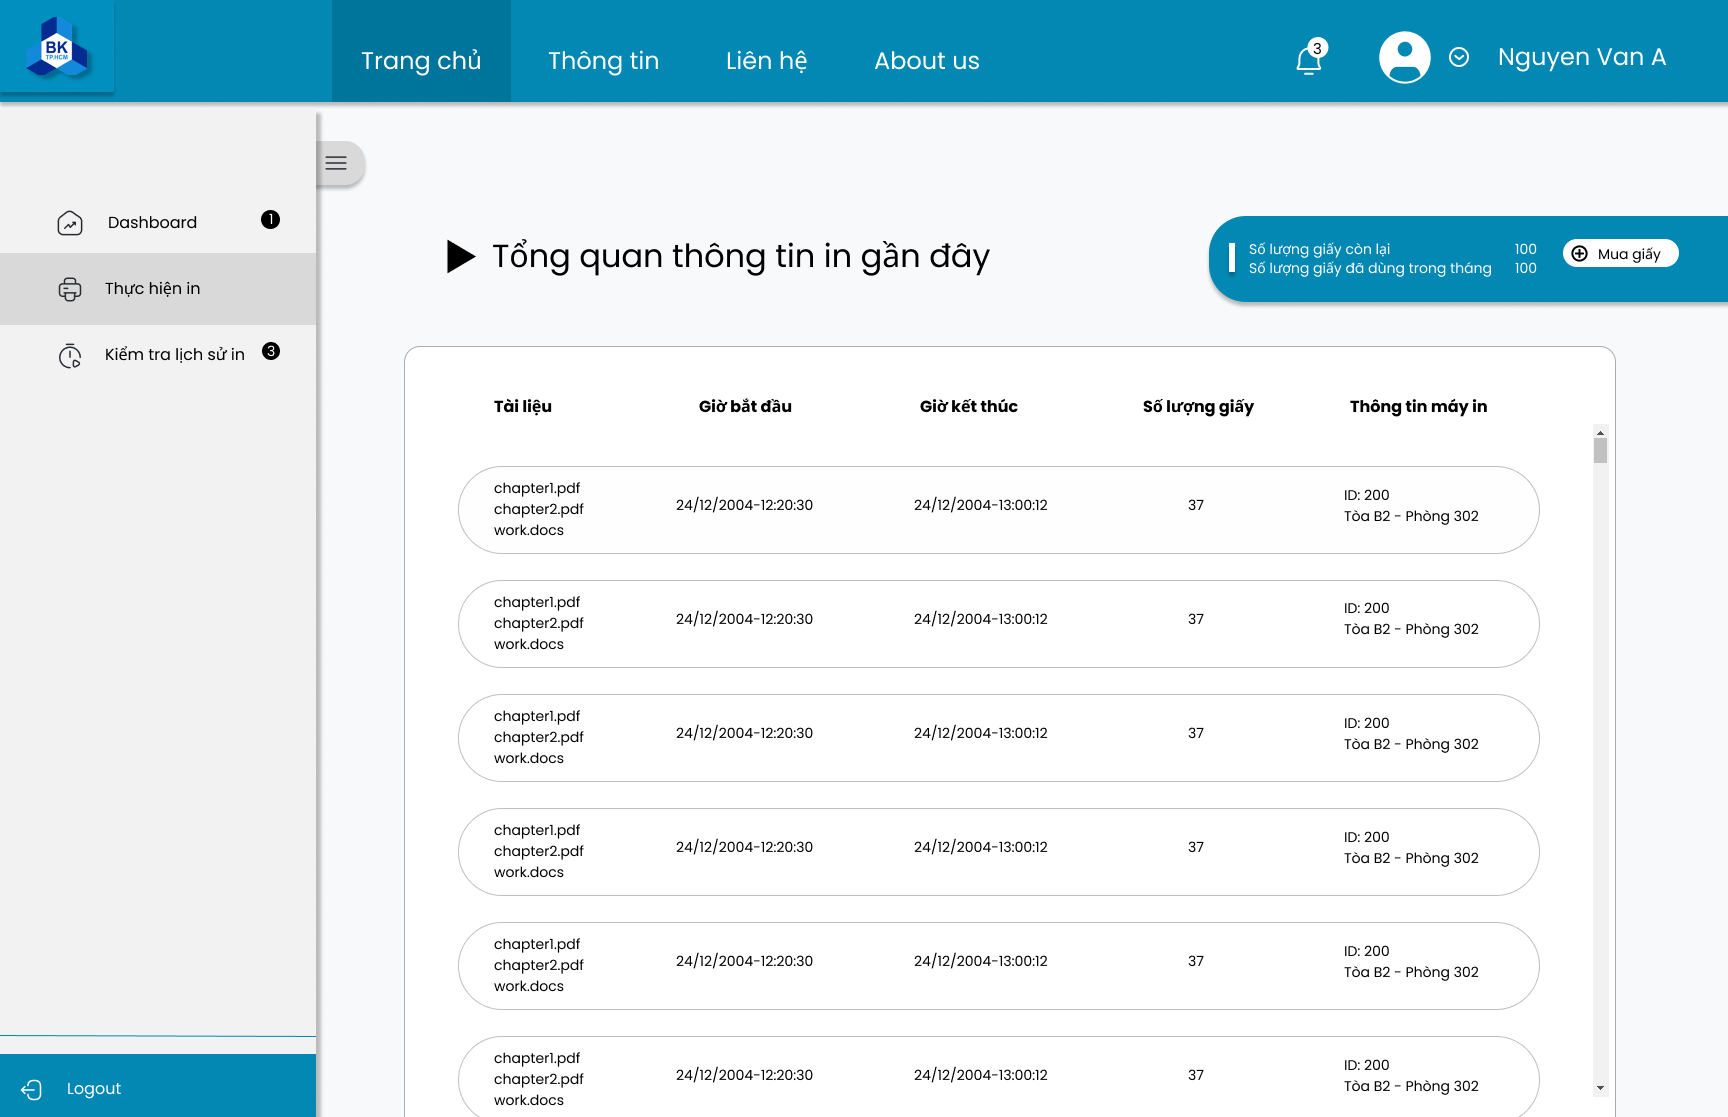
\includegraphics[width = 1\textwidth, ]{images/UI/Bảng điều khiển sinh viên.png}
    \caption{Student Dashboard Page}
\end{figure}  

\begin{figure}[H]
    \centering
    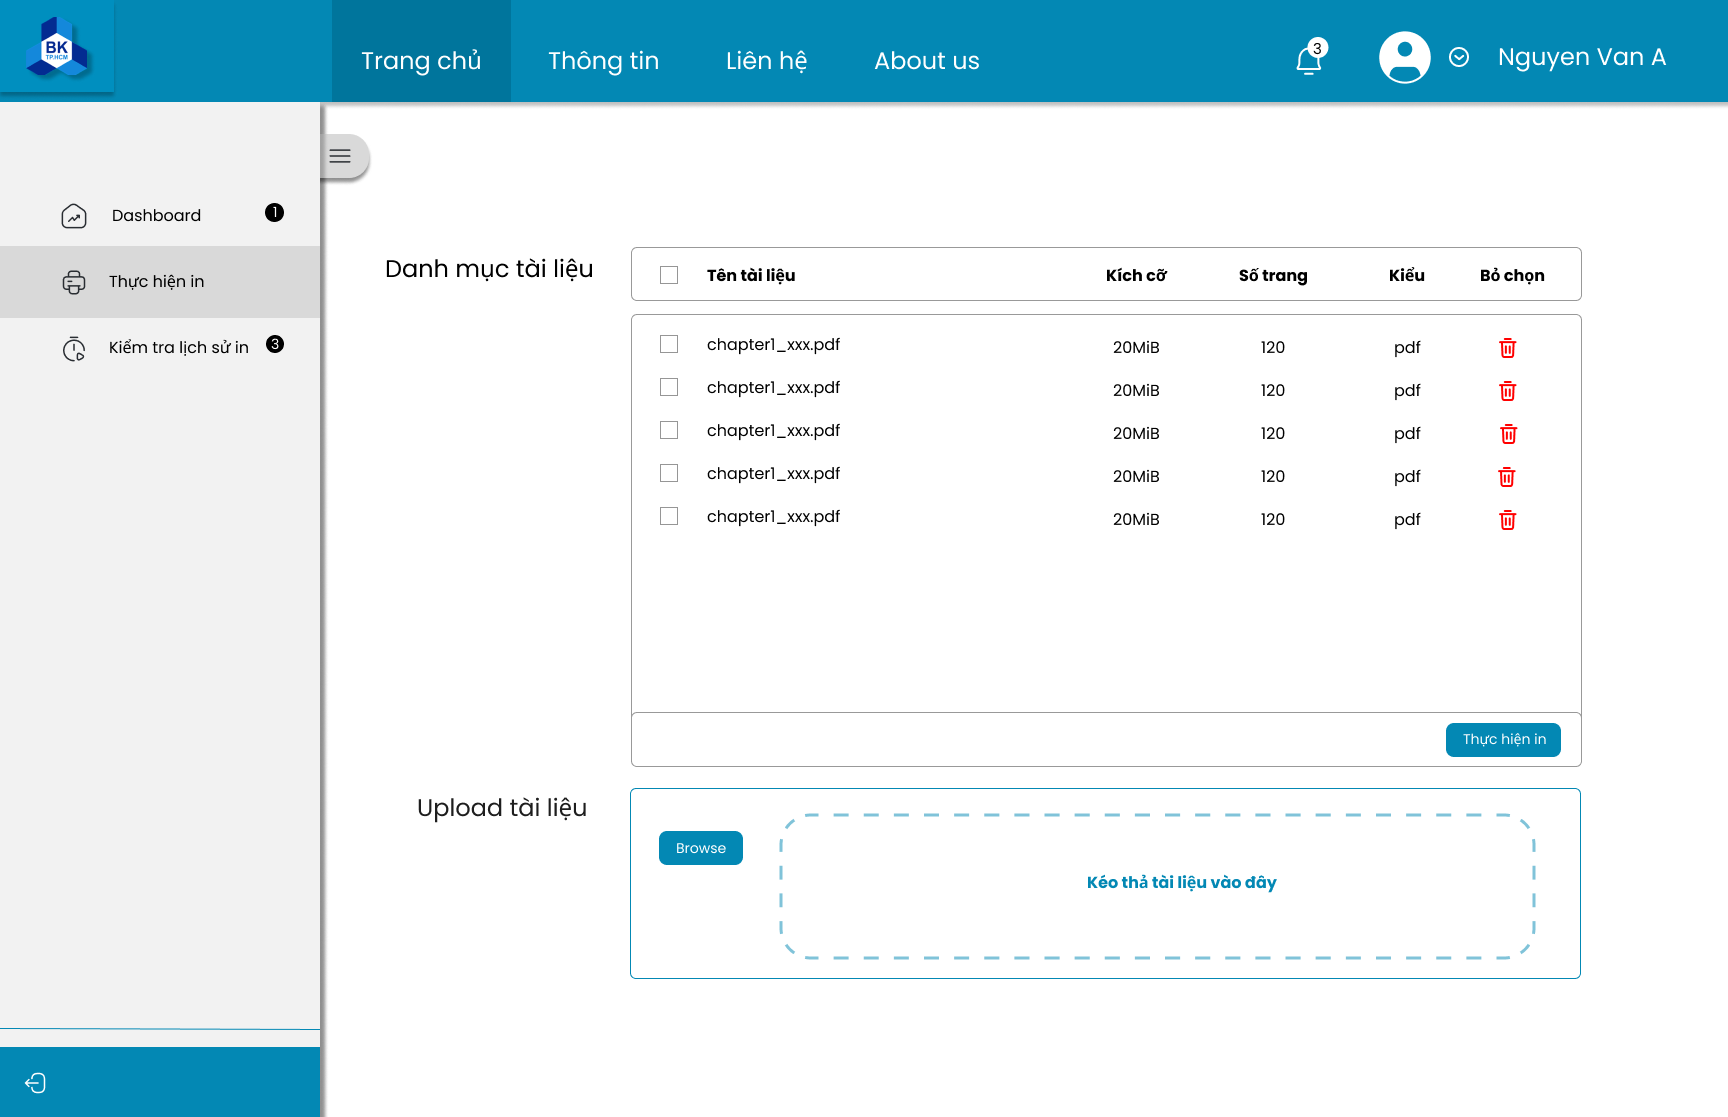
\includegraphics[width = \textwidth, ]{images/UI/Bảng in sinh viên.png}
    \caption{Student Printing Page}
\end{figure}  

\begin{figure}[H]
    \centering
    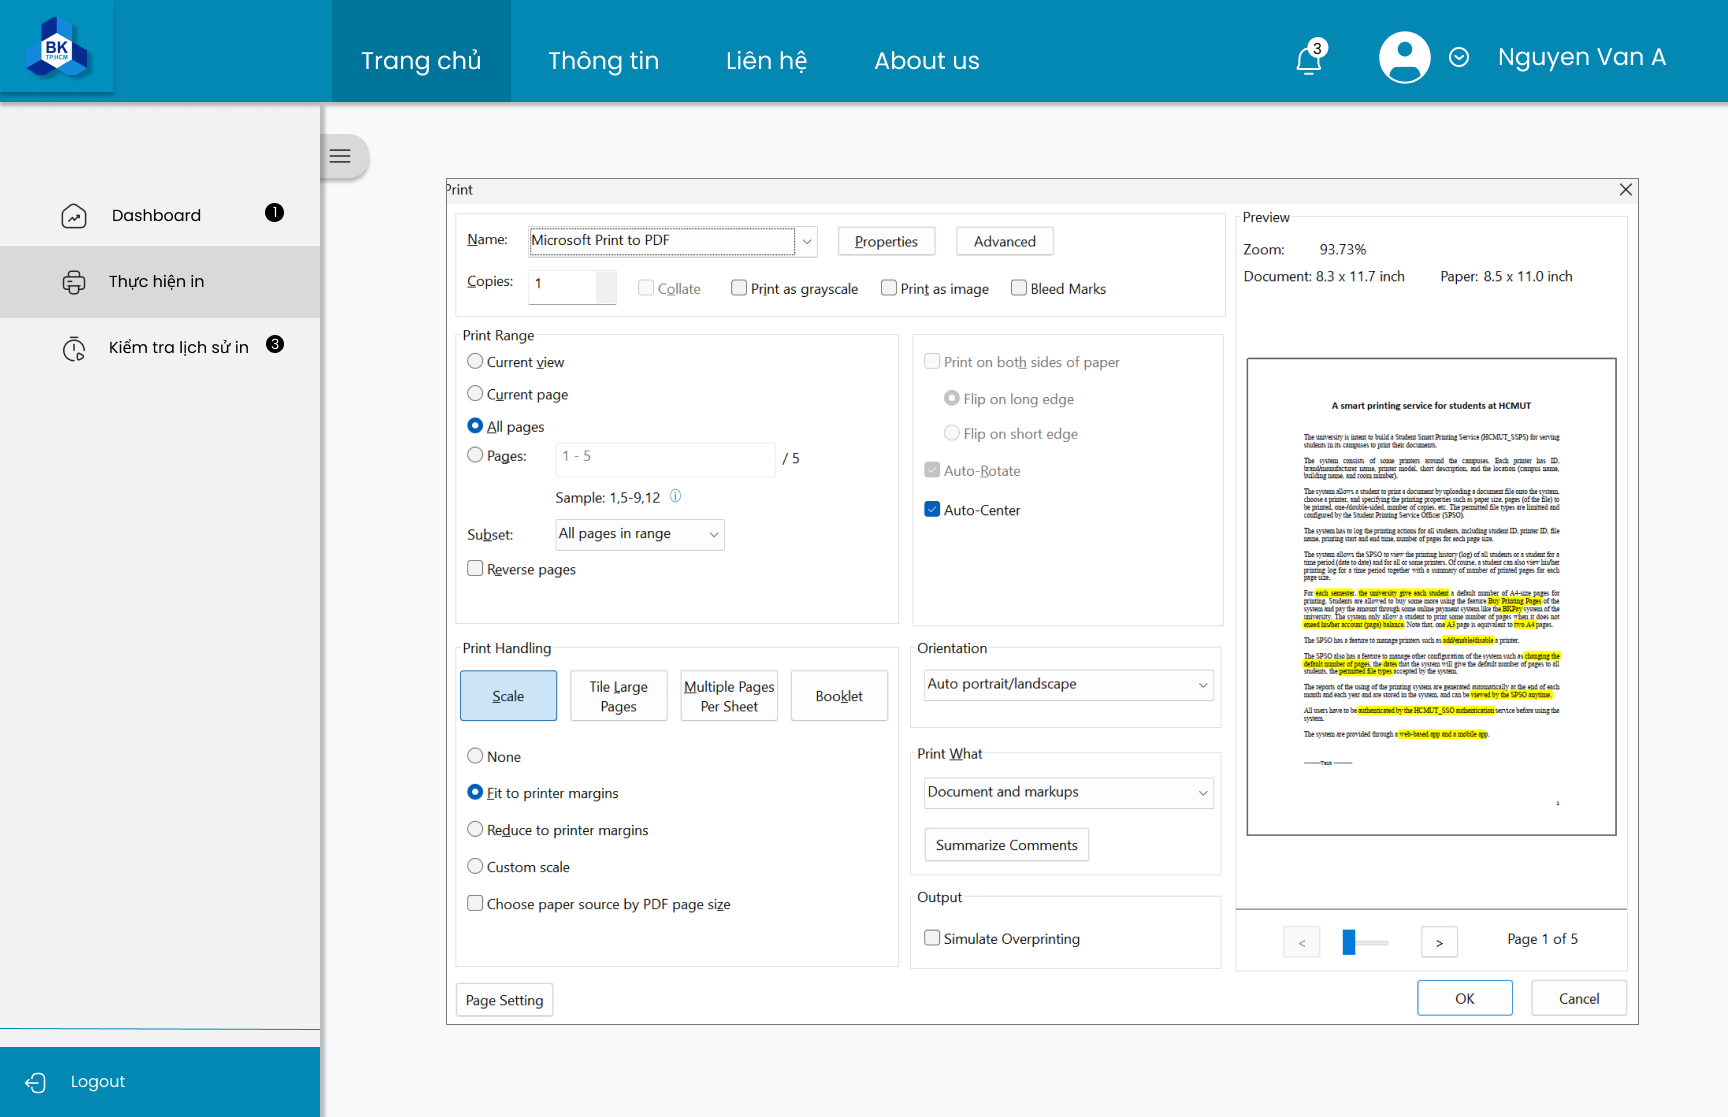
\includegraphics[width = \textwidth, ]{images/UI/Bảng in sinh viên 2.png}
    \caption{Student Printing Configuration Dialog}
\end{figure}  

\begin{figure}[H]
    \centering
    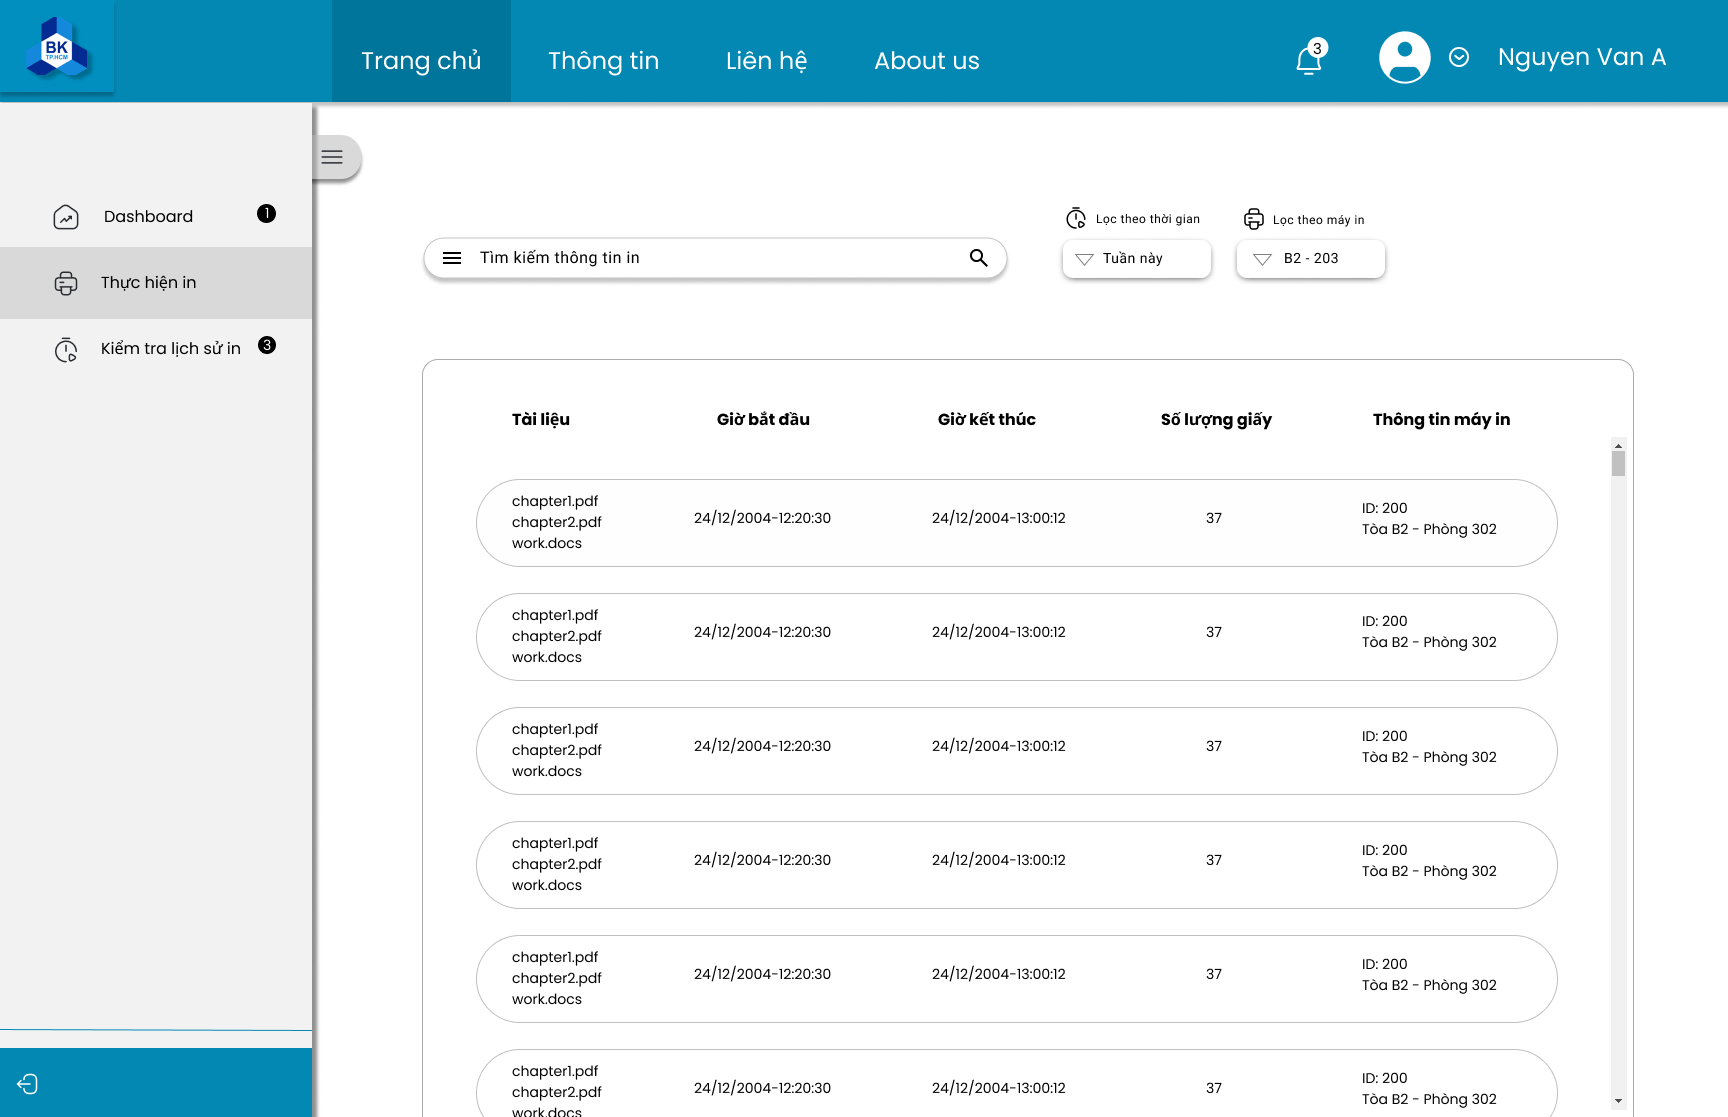
\includegraphics[width = \textwidth, ]{images/UI/Tra lịch sử sinh viên.png}
    \caption{Student History Log}
\end{figure}  

\begin{figure}[H]
    \centering
    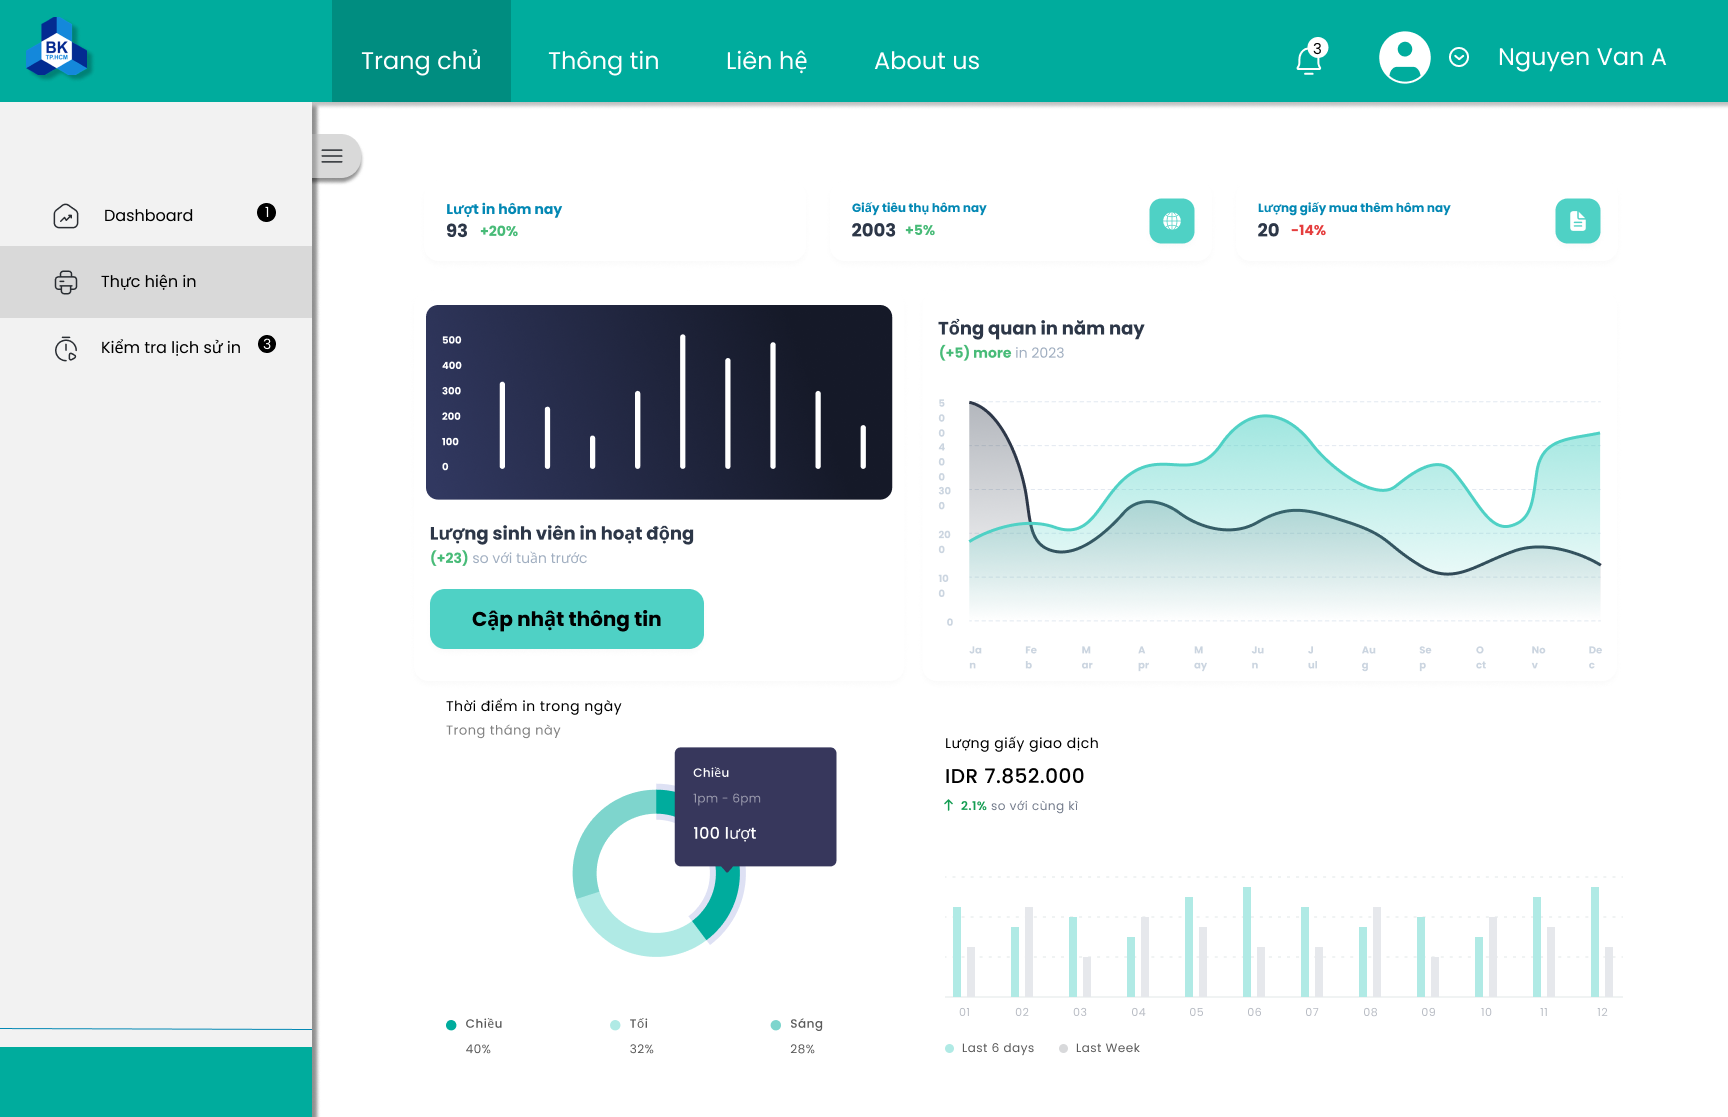
\includegraphics[width = \textwidth, ]{images/UI/Bảng điều khiển SPSO.png}
    \caption{SPSO Dashboard}
\end{figure}  

\begin{figure}[H]
    \centering
    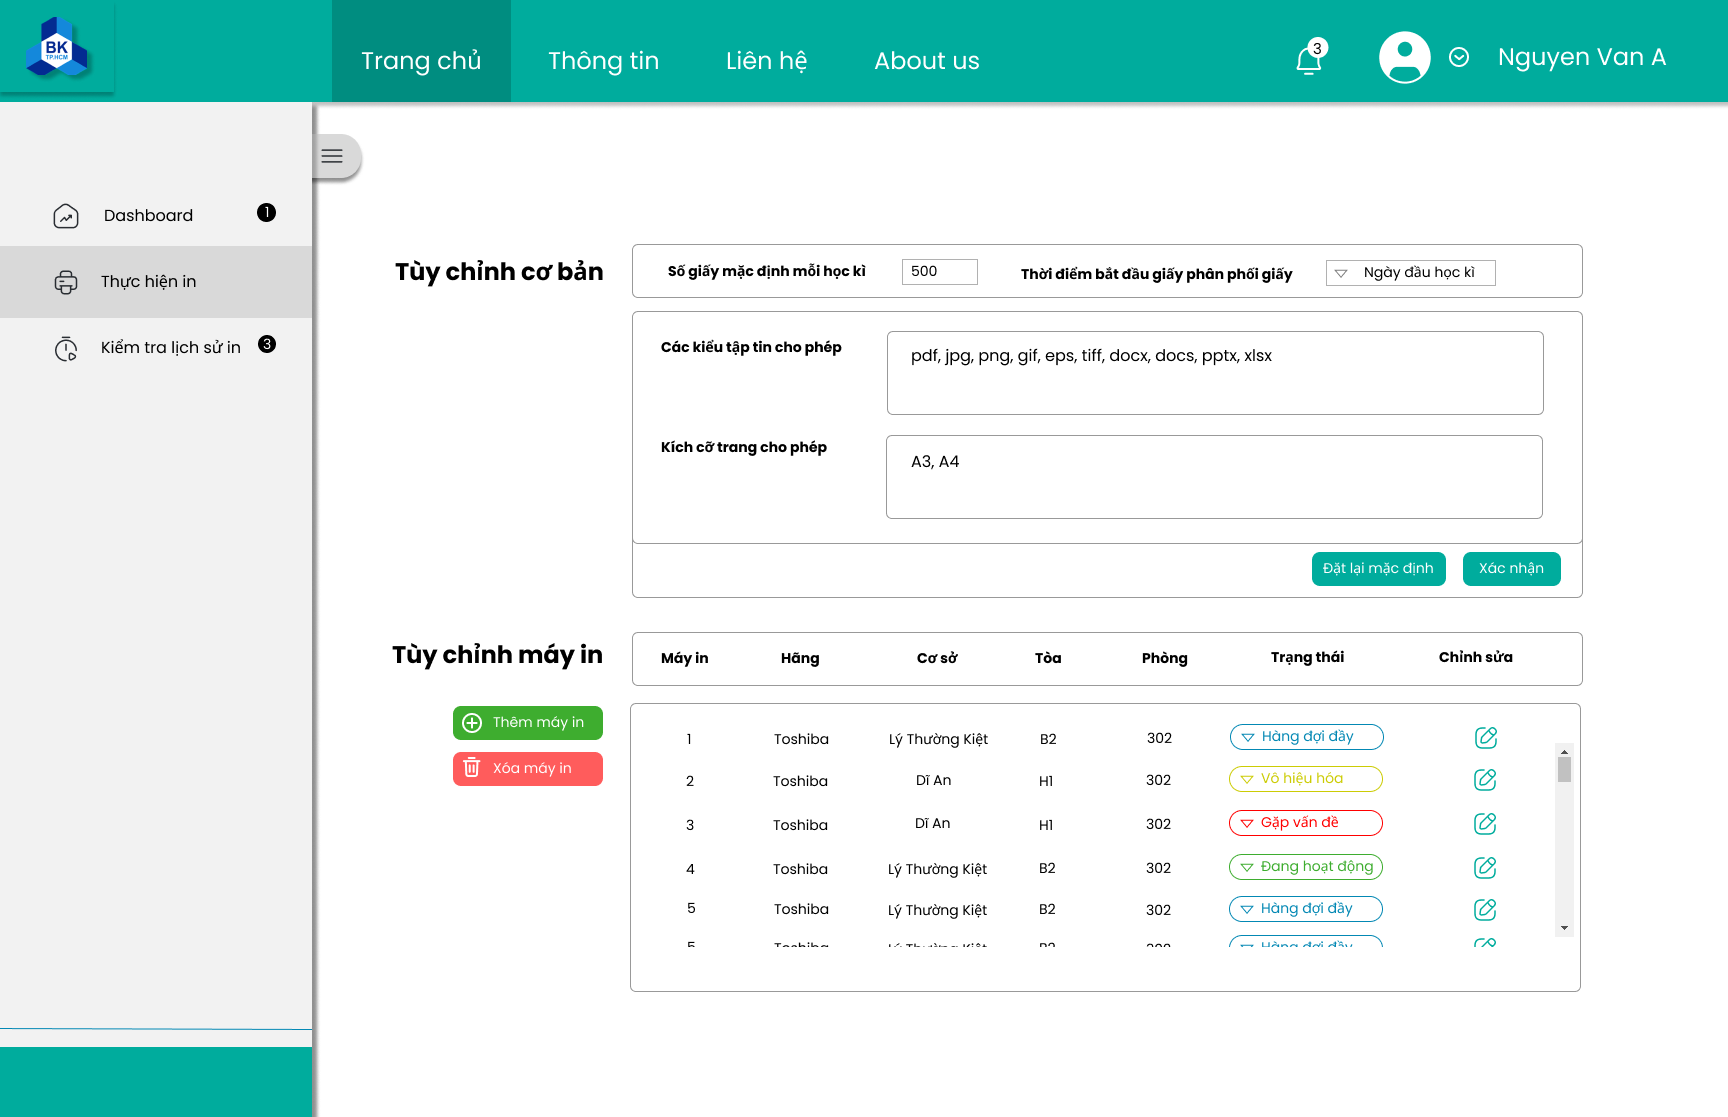
\includegraphics[width = \textwidth, ]{images/UI/Thay đổi in SPSO.png}
    \caption{SPSO Printing Configuration}
\end{figure}  

\begin{figure}[H]
    \centering
    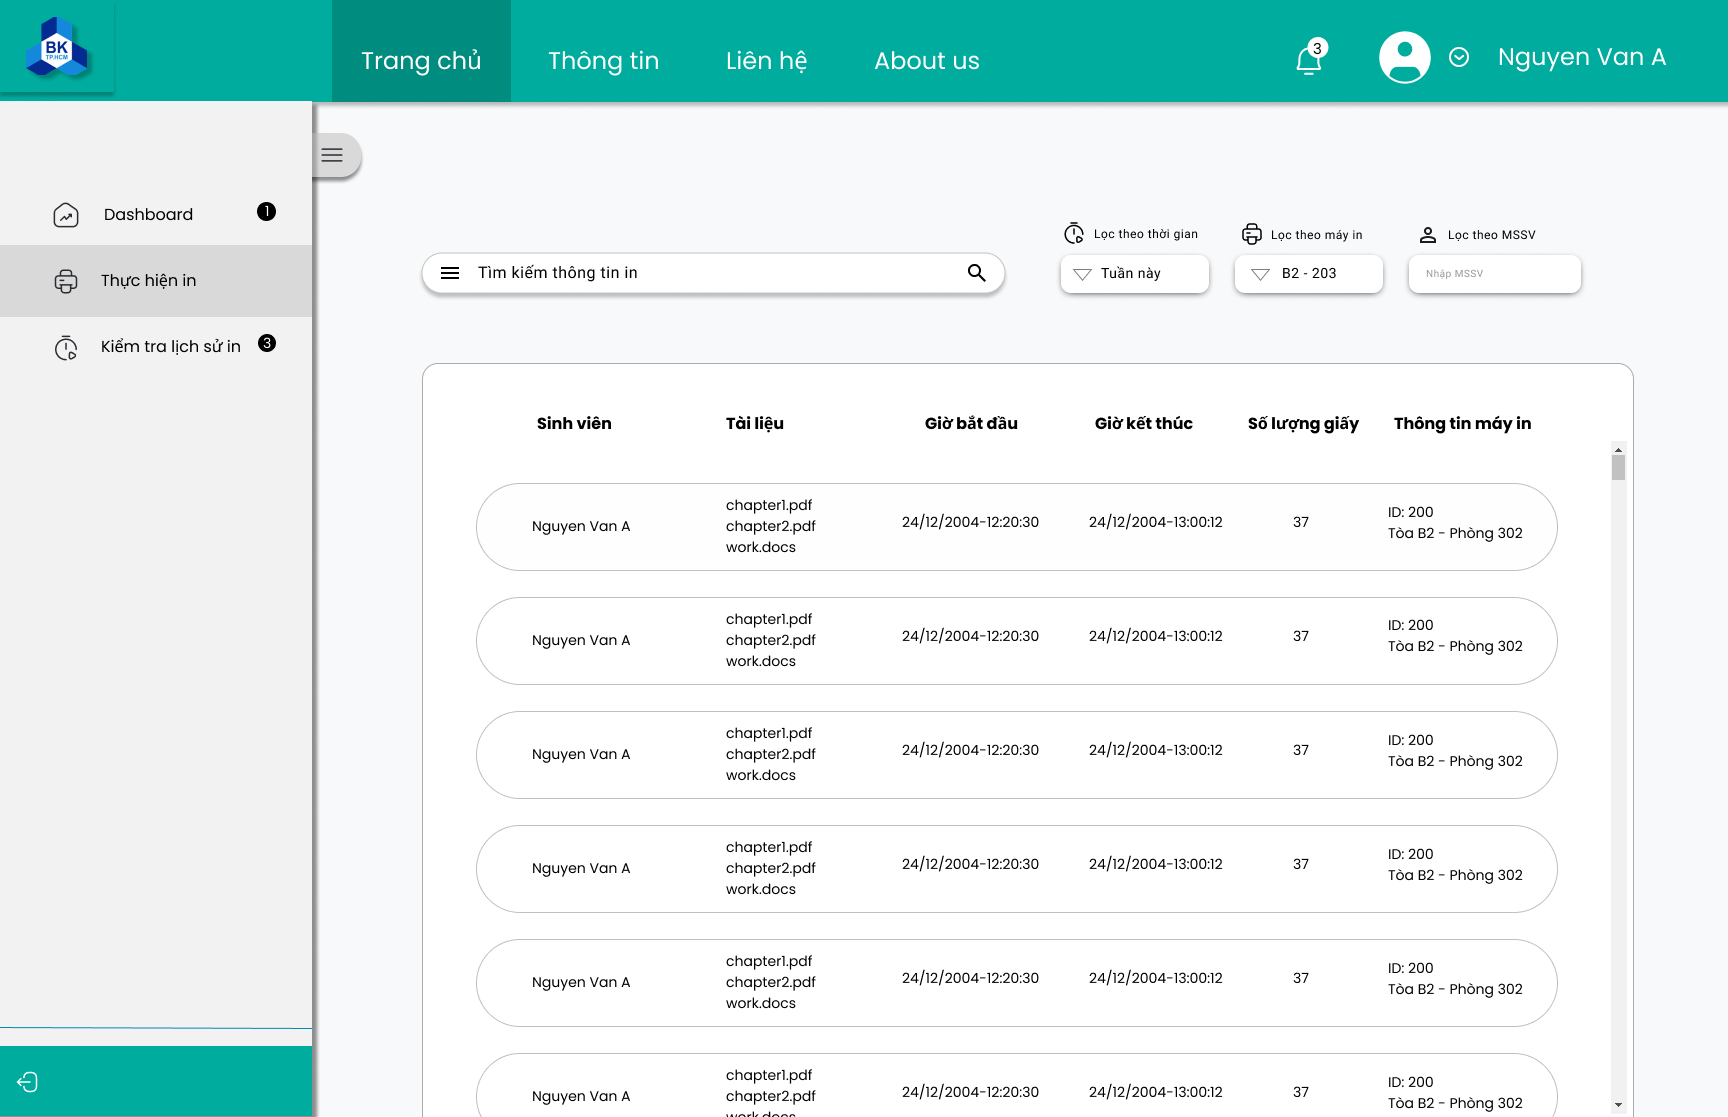
\includegraphics[width = \textwidth, ]{images/UI/Tra lịch sử SPSO.png}
    \caption{SPSO History Log}
\end{figure}  



\href{}{Link Figma}

\newpage